\documentclass[journal]{IEEEtai}

\usepackage[colorlinks,urlcolor=blue,linkcolor=blue,citecolor=blue]{hyperref}

% \usepackage{graphicx}%
% \usepackage{multirow}%
\usepackage{amsmath,amssymb,amsfonts}%
\usepackage{amsthm}%
\usepackage{mathrsfs}%
% \usepackage[title]{appendix}%
% \usepackage{xcolor}%
% \usepackage{textcomp}%
% \usepackage{manyfoot}%
% \usepackage{booktabs}%
% \usepackage{algorithm}%
% \usepackage{algorithmicx}%
% \usepackage{algpseudocode}%
% \usepackage{listings}%

\usepackage{hyperref}

%%%% For camera-ready, use this
%\documentclass[sigconf]{aamas}

\usepackage{listings}
\usepackage{xcolor}

\definecolor{codegreen}{rgb}{0,0.6,0}
\definecolor{codegray}{rgb}{0.5,0.5,0.5}
\definecolor{codepurple}{rgb}{0.58,0,0.82}
\definecolor{backcolour}{rgb}{0.95,0.95,0.92}
 
\lstdefinestyle{mystyle}{
    backgroundcolor=\color{backcolour},   
    commentstyle=\color{codegreen},
    keywordstyle=\color{magenta},
    numberstyle=\tiny\color{codegray},
    stringstyle=\color{codepurple},
    basicstyle=\footnotesize,
    breakatwhitespace=false,         
    breaklines=true,                 
    captionpos=b,                    
    keepspaces=true,                 
    numbers=left,                    
    numbersep=5pt,                  
    showspaces=false,                
    showstringspaces=false,
    showtabs=false,                  
    tabsize=2
}
 
\lstset{style=mystyle}

% --- Tickz
\usepackage{physics}
\usepackage{tikz}
\usepackage{amsmath}
\usepackage{mathdots}
% \usepackage{yhmath}
\usepackage{cancel}
\usepackage{color}
\usepackage{siunitx}
\usepackage{array}
\usepackage{multirow}
% \usepackage{amssymb}
\usepackage{gensymb}
\usepackage{tabularx}
\usepackage{extarrows}
\usepackage{booktabs}
\usetikzlibrary{fadings}
\usetikzlibrary{patterns}
\usetikzlibrary{shadows.blur}
\usetikzlibrary{shapes}

% ---------

\usepackage{balance} % for balancing columns on the final page
\usepackage{csquotes}
% \usepackage{cite}
\newcommand{\probP}{\text{I\kern-0.15em P}}
\usepackage{etoolbox}
\patchcmd{\thebibliography}{\section*{\refname}}{}{}{}
% \usepackage{amsthm,amssymb,amsfonts}

\usepackage[T1]{fontenc}
\usepackage{graphicx}
\usepackage{color}
% \renewcommand\UrlFont{\color{blue}\rmfamily}

\let\labelindent\relax
\usepackage[inline, shortlabels]{enumitem}
\usepackage{tabularx}
\usepackage{caption}
\usepackage{listings}
\usepackage{stfloats}
\usepackage{titlesec}
\usepackage{ragged2e}
% \usepackage[hyphens]{url}
\usepackage[linesnumbered,ruled,vlined]{algorithm2e}
\usepackage{float}
\usepackage[english]{babel}
\addto\extrasenglish{  
    \def\figureautorefname{Figure}
    \def\tableautorefname{Table}
    \def\algorithmautorefname{Algorithm}
    \def\sectionautorefname{Section}
    \def\subsectionautorefname{Subsection}
    \def\proofoutlineautorefname{Proof Outline}
}

%% \jvol{XX}
%% \jnum{XX}
%% \paper{1234567}
%% \pubyear{2020}
%% \publisheddate{xxxx 00, 0000}
%% \currentdate{xxxx 00, 0000}
%% \doiinfo{TQE.2020.Doi Number}

\newtheorem{theorem}{Theorem}
\newtheorem{lemma}{Lemma}
\setcounter{page}{1}
%% \setcounter{secnumdepth}{0}


\begin{document}


\title{Assisting Multi-Agent System Design with $\mathcal{M}OISE^+$ and MARL: The MAMAD Method} 


\author{Julien Soulé, Jean-Paul Jamont, Paul Théron, and Louis-Marie Traonouez,
\thanks{This work was primarily sent for peer-reviewing on the YYYY-DD-MM and was supported by Thales LAS and the AICA IWG}
\thanks{Julien Soulé, is with Grenoble INP, LCIS, Valence, France (e-mail: julien.soule@lcis.grenoble-inp.fr).}
\thanks{Jean-Paul Jamont, is with Grenoble INP, LCIS, Valence, France (e-mail: jean-paul.jamont@lcis.grenoble-inp.fr).}
\thanks{Michel Occello, is with Grenoble INP, LCIS, Valence, France (e-mail: michel.occello@lcis.grenoble-inp.fr).}
\thanks{Paul Théron, is with AICA IWG, Antibes, France (e-mail: paul.theron@orange.fr).}
\thanks{Louis-Marie Traonouez, is with Thales Land and Air Systems, BU IAS, Rennes, France (e-mail: louis-marie.traonouez@thalesgroup.com).}
\thanks{This paragraph will include the Associate Editor who handled your paper.}}

\markboth{Journal of IEEE Transactions on Artificial Intelligence, Vol. 00, No. 0, Month 2020}
{First A. Author \MakeLowercase{\textit{et al.}}: Bare Demo of IEEEtai.cls for IEEE Journals of IEEE Transactions on Artificial Intelligence}

\maketitle

\begin{abstract}
Designing Multi-Agent Systems (MAS) requires balancing structured agents' behaviors with adaptability. Traditional Agent-Oriented Software Engineering (AOSE) relies on expert knowledge, while Multi-Agent Reinforcement Learning (MARL) enables autonomous learning but lacks interpretability and control. By envisioning MAS design in general as finding proper agent's policies, then MARL enables finding suitable policies computationally, assisting in the AOSE design process. Yet, this idea of leveraging MARL for AOSE MAS design has not been largely explored to our knowledge.
%
To bridge this gap, we introduce \textbf{MOISE+MARL Assisted MAS Design (MAMAD)}, framing MAS design as an optimization problem under constraints, where a joint policy maximizes cumulative rewards while adhering to $\mathcal{M}OISE^+$ roles and goals. MAMAD follows a four-phase process:
1) \textbf{Modeling} the real-world environment,  
2) \textbf{Training} a policy under organizational specifications,  
3) \textbf{Analysis} of learnt behaviors,  
4) \textbf{Transfer} to real-world deployment.
%
We validate MAMAD in four case studies: Cyber-Defense scenario, Warehouse Management, Predator-Prey, and Overcooked-AI. Results show improved coordination, stability, and interpretability while reducing reliance on manual design efforts. MAMAD proposes a systematic approach to scalable, learning-driven MAS design.
\end{abstract}

\begin{IEEEImpStatement}
TODO: The impact statement should not exceeed 150 words. This section offers an example that is expanded to have only and just 150 words to demonstrate the point. Here is an example on how to write an appropriate impact statement: Chatbots are a popular technology in online interaction. They reduce the load on human support teams and offer continuous 24-7 support to customers. However, recent usability research has demonstrated that 30\% of customers are unhappy with current chatbots due to their poor conversational capabilities and inability to emotionally engage customers. The natural language algorithms we introduce in this paper overcame these limitations. With a significant increase in user satisfaction to 92\% after adopting our algorithms, the technology is ready to support users in a wide variety of applications including government front shops, automatic tellers, and the gaming industry. It could offer an alternative way of interaction for some physically disable users.
\end{IEEEImpStatement}

\begin{IEEEkeywords}
Agent-oriented Software Engineering, Multi-Agent Reinforcement Learning, Assisted-Design, Organizational Model
\end{IEEEkeywords}



\section{Introduction}

\subsection{Context}

Designing \textbf{MAS} for complex real-world applications, such as \textbf{cybersecurity}, \textbf{logistics}, \textbf{autonomous robotics}, and \textbf{intelligent transportation}, requires methodologies that ensure both \textbf{structured agent behaviors} and \textbf{agents' goals}~\cite{Jamont2O15}. Traditionally, the \textbf{Agent-oriented Software Engineering (AOSE)} paradigm has provided systematic frameworks for specifying and developing MAS, emphasizing the design of agents, roles, and interactions~\cite{Pavon2003, Bernon2005}. AOSE methodologies typically rely on explicit expert's knowledge and predefined organizational models to structure agent behavior, ensuring predictability, reliability, and adherence to system-wide constraints~\cite{Hindriks2014}.

Traditional AOSE approaches have significant \textbf{limitations in adaptability and scalability}. They often require extensive domain expertise to define organizational structures and behavioral rules, making them difficult to generalize across dynamic environments. To our knowledge, no work have carried out research pushing \textbf{machine learning (ML) capabilities} into AOSE MAS design, such as adaption to unforeseen events~\cite{Garcia2004}.

In contrast, \textbf{MARL} has emerged as a distinct ML approach that enables autonomous agents to \textbf{learn and adapt} through experience. MARL techniques allow agents to develop \textbf{coordination strategies} by interacting with their environment and optimizing their decision-making policies based on cumulative rewards~\cite{Zhang2021}. This data-driven learning paradigm enables agents to dynamically adjust their behaviors to different contexts, even in highly uncertain or complex environments, such as decentralized control, adversarial scenarios, or cooperative problem-solving~\cite{Papoudakis2021}.

From a theoretical perspective, integrating \textbf{MARL} into \textbf{AOSE} offers a promising pathway to enhance MAS design. MARL can assist by \textit{automatically determining agent policies} that align with environmental constraints and goals, reducing manual behavior specification. It may enable agents to \textit{learn coordination strategies} or \textit{adapt to changing environments} based on experience. In this view, MARL serves as a learning-driven layer that instantiates and operationalizes the abstractions defined in AOSE.

Despite its capabilities, MARL presents significant challenges in terms of \textbf{interpretability and control}. Unlike AOSE, which enforces structured agent interactions through predefined models, MARL relies on emergent behaviors, which can be unpredictable and difficult to interpret~\cite{Du2022}. This lack of transparency poses challenges in critical domains such as \textbf{cybersecurity} and \textbf{human-agent collaboration}, where ensuring explainability and adherence to high-level constraints is crucial. Furthermore, MARL lacks built-in mechanisms to enforce \textbf{organizational constraints}, such as predefined roles, team structures, or safety guidelines, limiting its applicability in mission-critical MAS applications~\cite{Nguyen2020}.

Given these contrasting advantages and limitations, this paper is positioned at finding a way to integrate the structured modeling capabilities of AOSE with the adaptive learning potential of MARL to design effective MAS, benefitting from the strengths of both domains.

% To enable the integration of MARL wihin AOSE, we aim an \textbf{approach} that unifies the strengths of both paradigms, providing a systematic way to \textbf{design MAS while enabling agents to learn and adapt within organizational constraints}.

\subsection{Problem statement and research gaps}

We adopt a optimization perspective on MAS design: we consider that designing a MAS in a deployment environment to achieve a global goal efficiently while adhering to optional additional user-defined requirements can be formulated as an \textbf{optimization problem under constraints in a MARL context}. In this formulation:
\begin{itemize}
    \item The \textbf{variable to optimize} is the agents' joint policy in the policy space ;
    \item The \textbf{goal function} is to maximize the cumulative reward over time, quantifying how effectively agents achieve their goal ;
    \item The \textbf{constraints} are the organizational specifications, such as user-defined roles and goals, representing the designer's requirements.
\end{itemize}
This formulation serves as the backbone of this article and motivates our contribution. 

To implement this approach, several key research gaps remain unaddressed when considering the design of MAS from an \textbf{organizational perspective}:
%
\begin{itemize}
  \item \textbf{(G1) Leveraging MARL's performance within AOSE}: AOSE lacks MARL integration, while MARL lacks structured design constraints. There is no \textbf{unified framework combining AOSE and MARL-driven learning}~\cite{Cossentino2014}. Addressing this gap would allow MAS to \textbf{leverage MARL's computational power} to optimize performance efficiently ;
  
  \item \textbf{(G2) Understanding emergent collective behaviors in MARL}: MARL agents develop unpredictable strategies, making behavior analysis difficult. A method is needed to \textbf{align emergent behaviors with organizational structures}~\cite{Du2022, Papoudakis2021}. Addressing this gap would improve \textbf{organizational explainability}, aiding validation, refinement, and deployment ;
  
  \item \textbf{(G3) Controlling or guiding agents at both individual and collective levels in MARL}: MARL lacks mechanisms to \textbf{guide agents toward structured behaviors while preserving flexibility}. Most approaches optimize performance without enforcing \textbf{organizational constraints}~\cite{Oroojlooy2023}. Addressing this gap would ensure \textbf{compliance with design requirements} and accelerate convergence by narrowing the policy search space ;
  
  \item \textbf{(G4) Automating end-to-end MAS design}: MAS design depends on domain experts and follows a costly, trial-and-error process. Manually crafted specifications \textbf{lack scalability and generalizability}~\cite{Nguyen2020}. Addressing this gap would enable \textbf{automated MAS design}, reducing expert reliance, manual effort, and resource costs while achieving comparable results.
\end{itemize}
%
These gaps highlight the need for a \textbf{method that integrates organizational modeling into MARL-driven MAS design}.


\subsection{Contributions and paper organization}

We propose the \textbf{MAMAD method}, which extends the proposed \textbf{MOISE+MARL} framework~\cite{soule2025moisemarl}, to structure MARL-driven learning. MAMAD enables \textbf{controlled policy learning}, aligning agents with predefined organizational specifications while extracting refined insights from emergent behaviors. It wraps the MOISE+MARL framework into a fully automated, four-phase design process driven by three key inputs: the environment, the user-defined design requirements, and the global goal. Each of these phases follows the optimization under the problem view.

In classical AOSE, the \textit{Requirement Engineering} phase refers to defining design requirements, environmental constraints, and global objectives~\cite{Pavon2003, Bernon2005}. We assume these inputs are already available and leave the choice of engineering methodology to the user. MAMAD then formalizes and operationalizes them within the MOISE+MARL framework as part of an automated design pipeline.

\begin{enumerate}
  \item \textbf{Modeling Phase:} Consists in modeling the "design problem" by automatically generating a simulated environment by training a neural network architecture akin to "world models"~\cite{Ha2018}; and the global MAS' goals as a reward function is defined to encapsulate the overarching goal of the system ;
  \item \textbf{Training Phase:} Agents are trained within the simulated environment, optionally incorporating organizational constraints in the form of roles (which restrict allowable actions) and goals (which adjust rewards to guide learning). These constraints serve as user-defined specifications to structure the learning process ;
  \item \textbf{Analysis Phase:} Unsupervised learning techniques are employed to analyze the trajectories of trained agents that successfully achieve their goals. This analysis aims to extract emergent roles and goals within the constrained policy space, ultimately yielding a validated set of organizational specifications and a joint policy ;
  \item \textbf{Transfer Phase:} The validated joint policy is deployed in the real-world environment, either remotely or directly, to operationalize the trained MAS ;
\end{enumerate}

We evaluated \textbf{MAMAD} in gamified environments, used as controlled testbeds to assess its effectiveness in conveniently generating high-fidelity simulation models during the Modeling phase. This approach bypasses the complexities of building simulations directly from physical environments.
Results demonstrated a clear alignment between the organizational specifications applied during training and those inferred agnostically in post-training analysis, validating both \textbf{explainability at the organizational level} and \textbf{compliance with design requirements}. Additionally, the generated MAS consistently achieved success rates on par with established benchmarks, confirming that \textbf{performance at achieving the goal} is preserved. Compared to manual design methods, \textbf{automation} was significantly improved, requiring fewer manual interventions. Ablation studies show that removing automated modeling reduced policy generalizability, while omitting organizational constraints resulted in erratic agent behaviors.

\

The remainder of this paper is organized as follows. \autoref{sec:related_works} reviews related work on MAS design, MARL, and organizational control, beginning with traditional AOSE methodologies and progressing to MARL-driven approaches. \autoref{sec:moise_marl} briefly recaps the \textbf{MOISE+MARL framework}, which serves as the foundation of our contribution. \autoref{sec:mamad} introduces the \textbf{MAMAD method}, detailing its design method. \autoref{sec:experimental_setup} describes the experimental setup, including the evaluation protocol, case studies, and baselines. \autoref{sec:results} presents and analyzes the experimental results. Finally, \autoref{sec:conclusion} summarizes our findings and discusses future research directions.

\clearpage

\section{Related works}\label{sec:related_works}

This section reviews existing research in MAS design, focusing on the intersection between AOSE and MARL. We structure this analysis into three topics. \autoref{sub-sec:aose_rel} presents AOSE methodologies and their limitations in addressing the identified gaps; \autoref{sub-sec:marl_rel} presents early MARL-driven approaches for MAS design; and \autoref{sub-sec:mm_rel} shows the underlying MOISE+MARL framework to bridge AOSE and MARL, though still lacking full design automation.

\subsection{AOSE methods for MAS design and their limitations}\label{sub-sec:aose_rel}

\textbf{AOSE} has introduced structured methodologies for MAS design, emphasizing role-based interactions, organizational hierarchies, and systematic agent coordination. Classical frameworks such as \textbf{GAIA}~\cite{gaia1998}, \textbf{ADELFE}~\cite{adelfe2002}, \textbf{INGENIAS}~\cite{ingenias2004}, and DIAMOND~\cite{Jamont2005} provide well-defined processes for designing MAS, relying on \textbf{explicit organizational modeling}. However, these methods are largely manual and require specialized knowledge to define agent behaviors, roles, and organizational constraints, making \textbf{scalability} in complex or dynamic environments cumbersome.

Although AOSE methodologies have explored \textbf{automation} in MAS design, such as \textbf{KB-Org}~\cite{kborg2001}, which offers templates to streamline organizational specification, no existing AOSE approach integrates \textbf{MARL} to automate learning-based MAS design. Consequently:
%
\begin{itemize}
    \item \textbf{(G1) Leveraging MARL's performance within AOSE} is entirely absent from AOSE ;
    \item \textbf{(G2) Understanding emergent collective behaviors in MARL} is not addressed, as AOSE methods rely on predefined rules rather than emergent learning ;
    \item \textbf{(G3) Controlling or guiding agents at both individual and collective levels in MARL} is not a focus of AOSE, since reinforcement learning is rarely incorporated ;
    \item \textbf{(G4) Automating end-to-end MAS design} is partially addressed (e.g., KB-Org) but remains highly manual and rule-driven.
\end{itemize}

Thus, while AOSE provides structured modeling tools, it lacks mechanisms for \textbf{adaptive learning}, \textbf{automated optimization}, and \textbf{MARL integration}, preventing it from fully addressing modern MAS design challenges.

\subsection{Early MARL-driven approaches for MAS design}\label{sub-sec:marl_rel}

Parallel to traditional AOSE, the field of \textbf{MARL} has introduced \textbf{data-driven} methods for MAS design, allowing agents to \textbf{autonomously learn} coordination strategies from experience. These approaches focus on \textbf{self-organizing agent behaviors}, often optimizing policies without explicit predefined organizational models.

% TODO: Donner plusieurs travaux + réfs et ne pas parler explicitement de Kim Hammar
One of the first attempts to apply MARL to MAS design is the work of \textbf{Kim Hammar}~\cite{hammar2019}, which proposes an \textbf{online framework} for Cybersecurity purposes where agents are trained in a simulation, using MARL to learn task-specific behaviors dynamically. This framework partially addresses:
%
\begin{itemize}
    \item \textbf{(G1) Leveraging MARL's performance within AOSE}, as it leverages reinforcement learning to structure MAS behavior ;
    \item \textbf{(G2) Understanding emergent collective behaviors in MARL}, offering visualization tools to interpret agent interactions, though without explicit organizational modeling ;
    \item \textbf{(G4) Automating end-to-end MAS design}, as Hammar's framework enables \textbf{online adaptation}, reducing manual effort.
\end{itemize}

However, these MARL-driven approaches remain \textbf{separate from AOSE} and do not provide mechanisms to explicitly model \textbf{organizational constraints}, leaving \textbf{(G3) Controlling or guiding agents at both individual and collective levels in MARL} largely unaddressed. Furthermore, while they improve \textbf{automation}, they lack structured \textbf{role-based design principles}, limiting their applicability in mission-critical MAS.

\subsection{Evaluating Organizational Fit}

Some works may be related to role or goal inference regarding the need to compute organizational fit or similar concepts.

Wilson et al.~\cite{wilson2008learning} develop a method for transferring roles in Multi-Agent MDPs, which helps agents adapt by transferring roles across different environments. However, their model lacks role abstraction as it focuses on specific, task-related roles rather than generalized organizational roles.

Berenji and Vengerov~\cite{berenji2000learning} investigate coordination and role inference in multi-agent systems, particularly in UAV missions, by enhancing cooperation through modeling agent dependencies. While useful for improving inter-agent cooperation, their approach remains task-specific and does not provide the abstract role computation required for organizational fit.

Yusuf and Baber~\cite{yusuf2020inferential} introduce inferential reasoning and Bayesian methods to facilitate task coordination among heterogeneous agents. While effective in dynamic coordination, their framework lacks a notion of role abstraction and does not measure alignment with a broader organizational structure.

Serrino et al.~\cite{serrino2019finding} examine dynamic role inference in social multi-agent environments, where agents deduce roles through interactions. While their approach enables flexible role understanding, it primarily focuses on immediate operational roles rather than abstract roles that align with long-term organizational models.

Recent advances in explainable reinforcement learning have sought to provide transparency in agent behavior. However, most approaches focus on making policies interpretable for humans~\cite{van2018explainable} rather than quantitatively assessing their alignment with predefined structural and functional organizations.

\

\noindent None of these works fully meet the requirements for abstract role computation or systematic organizational alignment. The concept of organizational fit proposed in this paper requires a framework that assesses alignment with predefined organizational structures and abstract goals.

\subsection{Controlling Organizational Fit}

Controlling organizational fit involves guiding agents to align their policies with predefined organizational structures, often through constraints, incentives, or structural enforcement.

Achiam et al.~\cite{achiam2017cpo} introduce Constrained Policy Optimization (CPO), which adjusts policies with safety constraints while maximizing rewards. MOISE+MARL extends this idea by introducing constraints beyond safety, shaping agent behavior toward predefined organizational expectations through externally guided learning.

Ray et al.~\cite{ray2019benchmarking} explore integrating constraints into reward functions using Lagrange multipliers, balancing the trade-off between reward maximization and constraint adherence. While this approach provides strong control, MOISE+MARL extends it by dynamically modifying both the action space and reward function, enforcing constraints at multiple levels to enable more flexible behavioral guidance.

Ensuring that agents learn while adhering to safety constraints is crucial in reinforcement learning. Garcia et al.~\cite{garcia2015comprehensive} provide a comprehensive survey of safe RL methods, highlighting their importance in preventing policy divergence. Alshiekh et al.~\cite{alshiekh2018safe} propose \textit{shielding}, a technique that blocks unsafe actions before execution. Unlike these approaches, MOISE+MARL leverages constraints to steer agents toward predefined roles rather than solely ensuring safety.

Hierarchical Reinforcement Learning (HRL) decomposes tasks into subtasks, aligning well with structured organizations. Ghavamzadeh et al.~\cite{ghavamzadeh2006hrl} demonstrate that HRL improves coordination in multi-agent settings. However, MOISE+MARL differs by imposing external organizational constraints rather than relying on a built-in hierarchical structure, enabling modular granularity in defining role-based constraints.

Foerster et al.~\cite{foerster2018communication} explore decentralized coordination through communication mechanisms that allow agents to operate collaboratively without explicit centralized control. While effective, these methods assume agents autonomously establish coordination rather than enforcing structured policies based on predefined organizational constraints.

\

\noindent Unlike HRL, the MOISE+MARL framework stands out for incorporating external organizational constraints that influence agents within a standard MARL framework, enabling structured yet adaptable agent behavior. Unlike Shielding or CPO, which primarily focus on safety constraints, MOISE+MARL introduces action modifications and reward shaping to enforce alignment with organizational roles. This structured yet adaptable approach enables scalable multi-agent systems where predefined role-based policies enhance both explainability and control.



% TODO: Faire un tableau récapitulatif des trois topics

\clearpage


\section{The MOISE+MARL Framework}
\label{sec:moise_marl_framework}

This section introduces the formalism used to describe the MOISE+MARL framework, which integrates organizational constraints into Multi-Agent Reinforcement Learning (MARL). Our approach builds upon the Decentralized Partially Observable Markov Decision Process (Dec-POMDP)~\cite{Oliehoek2016} framework and extends the $\mathcal{M}OISE^+$ organizational model~\cite{Hubner2007} to structure agent behaviors within a MARL environment.

\subsection{Markov Framework for MARL}
To apply MARL techniques, we rely on the \textit{Decentralized Partially Observable Markov Decision Process} (Dec-POMDP)~\cite{Beynier2013}, a formalism well-suited for multi-agent systems (MAS) in uncertain environments. Unlike \textit{Partially Observable Stochastic Games} (POSG), Dec-POMDP enforces a shared reward function across agents, fostering cooperation in joint policy learning~\cite{Albrecht2024}.

A Dec-POMDP $d \in D$ (where $D$ represents the set of Dec-POMDPs) is formally defined as a 7-tuple:
\begin{equation}
    d = (S, \{A_i\}, T, R, \{\Omega_i\}, O, \gamma)
\end{equation}
where:
\begin{itemize}
    \item $S$ is the finite set of states.
    \item $A_i$ represents the set of possible actions for agent $i$.
    \item $T: S \times A \times S \rightarrow [0,1]$ is the transition function defining state transitions.
    \item $R: S \times A \times S \rightarrow \mathbb{R}$ is the reward function.
    \item $\Omega_i$ is the observation space for agent $i$.
    \item $O: S \times A \times \Omega \rightarrow [0,1]$ defines the observation probabilities.
    \item $\gamma \in [0,1]$ is the discount factor controlling the weight of future rewards.
\end{itemize}

The objective in MARL is to find an optimal **joint policy** $\pi_{\text{joint}} = (\pi_1, \pi_2, \dots, \pi_n)$ that maximizes the cumulative expected reward:
\begin{equation}
    V^{\pi_{\text{joint}}}(s) = \mathbb{E} \left[ \sum_{t=0}^{\infty} \gamma^t R(s_t, a_t, s_{t+1}) \right].
\end{equation}

However, standard Dec-POMDPs do not inherently enforce structured agent behaviors. This motivates the integration of an **organizational model** to influence learning and ensure agents align with predefined roles and objectives.

\subsection{The $\mathcal{M}OISE^+$ Organizational Model}

\begin{figure}[h!]
    


\tikzset{every picture/.style={line width=0.75pt}} %set default line width to 0.75pt        

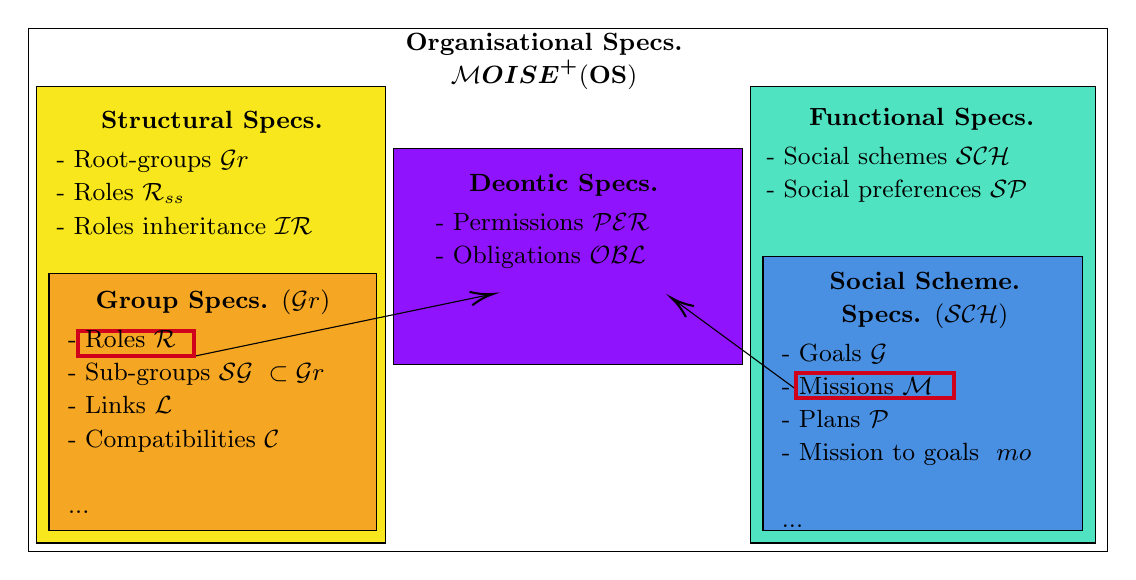
\begin{tikzpicture}[x=0.75pt,y=0.75pt,yscale=-1,xscale=1]
%uncomment if require: \path (0,1656); %set diagram left start at 0, and has height of 1656

%Shape: Rectangle [id:dp6756844921493015] 
\draw  [fill={rgb, 255:red, 248; green, 231; blue, 28 }  ,fill opacity=1 ] (46,1204) -- (214,1204) -- (214,1424) -- (46,1424) -- cycle ;
%Shape: Rectangle [id:dp3759944257810566] 
\draw  [fill={rgb, 255:red, 80; green, 227; blue, 194 }  ,fill opacity=1 ] (390,1204) -- (556,1204) -- (556,1424) -- (390,1424) -- cycle ;
%Shape: Rectangle [id:dp28244406216006945] 
\draw  [fill={rgb, 255:red, 144; green, 19; blue, 254 }  ,fill opacity=1 ] (218,1234) -- (386,1234) -- (386,1338) -- (218,1338) -- cycle ;
%Shape: Rectangle [id:dp32232123359581766] 
\draw   (42,1176) -- (562,1176) -- (562,1428) -- (42,1428) -- cycle ;
%Shape: Rectangle [id:dp7605706269262755] 
\draw  [fill={rgb, 255:red, 74; green, 144; blue, 226 }  ,fill opacity=1 ] (396,1286) -- (550,1286) -- (550,1418) -- (396,1418) -- cycle ;
%Shape: Rectangle [id:dp33110985390647496] 
\draw   (52,1294) -- (210,1294) -- (210,1418) -- (52,1418) -- cycle ;
%Shape: Rectangle [id:dp8653560038381976] 
\draw  [fill={rgb, 255:red, 245; green, 166; blue, 35 }  ,fill opacity=1 ] (52,1294) -- (210,1294) -- (210,1418) -- (52,1418) -- cycle ;
%Straight Lines [id:da09781093164567278] 
\draw    (412,1350) -- (353.61,1307.18) ;
\draw [shift={(352,1306)}, rotate = 36.25] [color={rgb, 255:red, 0; green, 0; blue, 0 }  ][line width=0.75]    (10.93,-3.29) .. controls (6.95,-1.4) and (3.31,-0.3) .. (0,0) .. controls (3.31,0.3) and (6.95,1.4) .. (10.93,3.29)   ;
%Straight Lines [id:da3938396723807833] 
\draw    (122,1334) -- (264.04,1304.41) ;
\draw [shift={(266,1304)}, rotate = 168.23] [color={rgb, 255:red, 0; green, 0; blue, 0 }  ][line width=0.75]    (10.93,-3.29) .. controls (6.95,-1.4) and (3.31,-0.3) .. (0,0) .. controls (3.31,0.3) and (6.95,1.4) .. (10.93,3.29)   ;
%Shape: Rectangle [id:dp269311335478327] 
\draw  [color={rgb, 255:red, 208; green, 2; blue, 27 }  ,draw opacity=1 ][line width=1.5]  (66,1322) -- (122,1322) -- (122,1334) -- (66,1334) -- cycle ;
%Shape: Rectangle [id:dp7449860119164387] 
\draw  [color={rgb, 255:red, 208; green, 2; blue, 27 }  ,draw opacity=1 ][line width=1.5]  (412,1342) -- (488,1342) -- (488,1354) -- (412,1354) -- cycle ;


% Text Node
\draw (472.5,1237.41) node   [align=left] {\begin{minipage}[lt]{112.2pt}\setlength\topsep{0pt}
\begin{center}
\textbf{{\small Functional Specs.}}
\end{center}
{\small  - Social schemes $\displaystyle \mathcal{SCH}$}\\{\small  - Social preferences $\displaystyle \mathcal{SP}$}
\end{minipage}};
% Text Node
\draw (474,1355) node   [align=left] {\begin{minipage}[lt]{103.36pt}\setlength\topsep{0pt}
\begin{center}
\textbf{{\small Social Scheme.}}\\{\small \textbf{Specs. }$\displaystyle (\mathcal{SCH})$}
\end{center}
{\small  - Goals $\displaystyle \mathcal{G}$}\\{\small  - Missions $\displaystyle \mathcal{M}$}\\{\small  - Plans $\displaystyle \mathcal{P}$}\\{\small  - Mission to goals \ $\displaystyle mo$}\\\\{\small  ...}
\end{minipage}};
% Text Node
\draw (131,1356) node   [align=left] {\begin{minipage}[lt]{104.72pt}\setlength\topsep{0pt}
\begin{center}
{\small \textbf{Group Specs. }$\displaystyle (\mathcal{G} r)$}
\end{center}
{\small  - Roles $\displaystyle \mathcal{R}$}\\{\small  - Sub-groups $\displaystyle \mathcal{SG} \ \subset \mathcal{G} r$}\\{\small  - Links $\displaystyle \mathcal{L}$}\\{\small  - Compatibilities $\displaystyle \mathcal{C}$}\\\\{\small  ...}
\end{minipage}};
% Text Node
\draw (181,1177) node [anchor=north west][inner sep=0.75pt]   [align=left] {\begin{minipage}[lt]{162.41pt}\setlength\topsep{0pt}
\begin{center}
{\small \textbf{Organisational Specs. }$\displaystyle \mathcal{M}\boldsymbol{OISE^{+}}$($\displaystyle \mathbf{OS}$)}
\end{center}

\end{minipage}};
% Text Node
\draw (300,1269.09) node   [align=left] {\begin{minipage}[lt]{92.48pt}\setlength\topsep{0pt}
\begin{center}
\textbf{{\small Deontic Specs.}}
\end{center}
{\small  - Permissions $\displaystyle \mathcal{PER}$}\\{\small  - Obligations $\displaystyle \mathcal{OBL}$}
\end{minipage}};
% Text Node
\draw (130.5,1245.69) node   [align=left] {\begin{minipage}[lt]{112.2pt}\setlength\topsep{0pt}
\begin{center}
\textbf{{\small Structural Specs.}}
\end{center}
{\small  - Root-groups $\displaystyle \mathcal{G} r$}\\{\small  - Roles $\displaystyle \mathcal{R}_{ss}$}\\{\small  - Roles inheritance $\displaystyle \mathcal{IR}$}
\end{minipage}};


\end{tikzpicture}
    \caption{A synthetic view of the $\mathcal{M}OISE^+$ model}
    \label{fig:moise_model}
\end{figure}

The $\mathcal{M}OISE^+$ organizational model~\cite{Hubner2007} provides a structured approach to multi-agent organization, facilitating the enforcement of role-based constraints in MARL. As illustrated in \autoref{fig:moise_model}, $\mathcal{M}OISE^+$ consists of three core specifications:

\noindent \textbf{1. Structural Specifications (SS)} define agent relationships and roles within the system:
\begin{equation}
    \mathcal{SS} = \langle \mathcal{R}, \mathcal{IR}, \mathcal{G} \rangle.
\end{equation}
where:
\begin{itemize}
    \item $\mathcal{R}$ is the set of roles.
    \item $\mathcal{IR}$ defines inheritance relationships among roles.
    \item $\mathcal{G}$ is the set of organizational groups.
\end{itemize}

\noindent \textbf{2. Functional Specifications (FS)} describe goal-oriented agent behaviors:
\begin{equation}
    \mathcal{FS} = \langle \mathcal{SCH}, \mathcal{PO} \rangle.
\end{equation}
where:
\begin{itemize}
    \item $\mathcal{SCH}$ structures global goals, missions, and plans.
    \item $\mathcal{PO}$ represents mission preferences and execution priorities.
\end{itemize}

\noindent \textbf{3. Deontic Specifications (DS)} enforce role-based permissions and obligations:
\begin{equation}
    \mathcal{DS} = \langle \mathcal{OBL}, \mathcal{PER} \rangle.
\end{equation}
where:
\begin{itemize}
    \item $\mathcal{OBL}$ denotes mandatory role assignments.
    \item $\mathcal{PER}$ specifies optional role permissions.
\end{itemize}

\subsection{Linking $\mathcal{M}OISE^+$ with MARL}

We introduce **Constraint Guides** to bridge the gap between $\mathcal{M}OISE^+$ and MARL, enabling structured policy learning. These guides enforce agent behavior through modifications to action spaces and rewards.

\noindent \textbf{1. Role Action Guide (RAG)}: Limits action choices based on predefined role constraints:
\begin{equation}
    rag: H \times \Omega \rightarrow \mathcal{P}(A \times \mathbb{R}).
\end{equation}

\noindent \textbf{2. Role Reward Guide (RRG)}: Penalizes deviations from expected role-based behaviors:
\begin{equation}
    rrg: H \times \Omega \times A \rightarrow \mathbb{R}.
\end{equation}

\noindent \textbf{3. Goal Reward Guide (GRG)}: Encourages alignment with predefined goal trajectories:
\begin{equation}
    grg: H \rightarrow \mathbb{R}.
\end{equation}

Additionally, we define \textbf{Linkers} to connect $\mathcal{M}OISE^+$ structures with MARL:
\begin{itemize}
    \item \textbf{Agent to Role} ($ar: \mathcal{A} \to \mathcal{R}$) assigns roles to agents.
    \item \textbf{Role to Constraint Guide} ($rcg: \mathcal{R} \rightarrow rag \cup rrg$) links roles to action and reward constraints.
    \item \textbf{Goal to Constraint Guide} ($gcg: \mathcal{G} \rightarrow grg$) associates goals with reward incentives.
\end{itemize}

\autoref{fig:mm_synthesis} illustrates the overall MOISE+MARL framework, integrating $\mathcal{M}OISE^+$ specifications with constraint-guided MARL training.

\subsection{Solving the MOISE+MARL Problem}

The goal is to find an optimal joint policy $\pi^j$ that maximizes the modified state-value function:
\begin{equation}
    V^{\pi^{j}}(s_t) = \sum_{a_t \in A_t} \pi^j(a_t | \omega_t) \sum_{s_{t+1} \in S} T(s_{t+1} | s_t, a_t) [R' + V^{\pi^{j}}(s_{t+1})].
\end{equation}
where:
\begin{equation}
    R' = R(s_t, a_t, s_{t+1}) + grg(h_t) - rrg(h_t, \omega_t, a_t).
\end{equation}

This formulation ensures that agents **adhere to organizational roles** while optimizing performance in MARL.

\subsection{Implementation Considerations}
Implementing constraint guides manually is tedious. To simplify this, we introduce **Trajectory-based Patterns (TPs)**, inspired by NLP methods, to encode behavioral constraints. A TP $p \in P$ is defined as:
\begin{equation}
    p = \langle h, (c_{\text{min}}, c_{\text{max}}) \rangle.
\end{equation}
where $h$ represents a sequence of observations/actions, and $(c_{\text{min}}, c_{\text{max}})$ defines repetition constraints.

By leveraging these patterns, constraint enforcement becomes more interpretable and scalable. The MOISE+MARL framework enables structured MARL training through the integration of the $\mathcal{M}OISE^+$ organizational model.


\section{The TEMM Method}
\label{sec:TEMM_algorithm}

As presented in \autoref{sec:related_works}, no existing method fully meets our requirements for determining abstract roles, abstract goals, or organizational fit. To address this gap, we propose the \textbf{Trajectory-based Evaluation in MOISE+MARL} (TEMM) method for the automatic inference and evaluation of roles and missions based on observed behaviors over multiple episodes.

\

\noindent TEMM leverages unsupervised learning techniques to generalize abstract roles and missions from observed behaviors across multiple test episodes. By measuring the deviation between inferred abstract organizational specifications and actual agent behaviors, TEMM quantifies \textit{organizational fit}, providing a measure of how well a policy aligns with inferred abstract organizational structures.

\subsection{Formalizing Organizational Inference in TEMM}

TEMM is based on a set of definitions that link $\mathcal{M}OISE^+$ organizational specifications to observed joint histories. Each specification is inferred using dedicated unsupervised learning techniques that progressively build an abstract organization based on agent behaviors.

\noindent The TEMM method follows a three-step process:
\begin{enumerate}
    \item **Inferring roles and their inheritance** using hierarchical clustering.
    \item **Inferring goals, plans, and missions** using trajectory clustering and observation-state analysis.
    \item **Inferring obligations and permissions** by analyzing temporal constraints and goal consistency.
\end{enumerate}

\noindent The following sections detail each of these steps.
%
\footnotetext[1]{ \label{fn:github} Additional details, developed code, datasets, and hyperparameter configurations are available at \url{https://github.com/julien6/MOISE-MARL}.}

\subsection{Inferring Roles and Their Inheritance}

We define a \textbf{role} $\rho$ as a set of policies whose associated agent histories share a \textbf{Common Longest Subsequence (CLS)}. A role $\rho_2$ is considered a \textbf{sub-role} of $\rho_1$ if the CLS of histories associated with $\rho_2$ is contained within that of $\rho_1$. This definition formalizes role abstraction in MARL.

To infer roles, TEMM applies a \textit{hierarchical clustering} algorithm to identify CLSs across agent histories:
\begin{equation}
    \rho = \text{argmax}_{\rho} \left( \sum_{h \in H_{\rho}} | \text{CLS}(h, H_{\rho}) | \right),
\end{equation}
where $\text{CLS}(h, H_{\rho})$ is the longest common sequence among histories in role $\rho$.

A \textbf{dendrogram} representation of clustering results allows for the visualization of inferred hierarchical role structures. Given the hierarchical nature of CLS extraction, TEMM recursively partitions histories into increasingly abstract roles, ensuring organizational coherence.

\noindent **Measuring Structural Organizational Fit:**  
TEMM computes the alignment between agent trajectories and inferred abstract roles:
\begin{equation}
    \text{Structural Fit} = \frac{1}{|H|} \sum_{h \in H} \frac{| \text{CLS}(h, H_{\rho(h)}) |}{|h|}.
\end{equation}

\subsection{Inferring Goals, Plans, and Missions}

A \textbf{goal} is defined as a recurring set of joint observations reached by successful agents following their trajectories. A \textbf{mission} consists of a set of goals collectively achieved by an agent.

To infer goals, TEMM follows these steps:
\begin{enumerate}
    \item Compute a \textbf{joint-observation transition graph} for each joint-history.
    \item Merge transition graphs into a general \textbf{global transition model}.
    \item Cluster observation sequences using \textbf{K-means} to identify trajectory patterns.
    \item Sample key joint-observations as \textbf{abstract goals}.
\end{enumerate}

A goal $g$ is identified as:
\begin{equation}
    g = \text{argmin}_{o \in \Omega} \left( \sum_{h \in H} d_{\text{traj}}(o, H) \right),
\end{equation}
where $d_{\text{traj}}(o, H)$ represents the variance of joint-observations $o$ across all agent trajectories.

Using the inferred goals, TEMM reconstructs \textbf{plans} by identifying sequential dependencies:
\begin{equation}
    p = \{ (g_i, g_j) \ | \ g_j \text{ follows } g_i \text{ in at least } k\% \text{ of episodes} \}.
\end{equation}

A \textbf{mission} is defined as the set of goals pursued by an agent over multiple episodes:
\begin{equation}
    m = \{ g_1, g_2, \dots, g_n \}, \quad \forall g_i \in G, P(m | G) > \theta.
\end{equation}

\noindent **Measuring Functional Organizational Fit:**  
To measure how well a policy conforms to inferred abstract goals:
\begin{equation}
    \text{Functional Fit} = \frac{1}{|H|} \sum_{h \in H} \frac{| g(h) \cap G |}{| G |}.
\end{equation}

\subsection{Inferring Obligations and Permissions}

An \textbf{obligation} exists when an agent, playing role $\rho$, exclusively fulfills the goals of a mission $m$ within a given time frame. A \textbf{permission} is granted when an agent may accomplish other goals outside of its mission.

TEMM determines obligations and permissions by:
\begin{enumerate}
    \item Identifying agent-to-mission associations.
    \item Checking whether an agent's behavior remains within predefined time constraints.
    \item Analyzing deviations from inferred mission structures.
\end{enumerate}

A role $\rho$ is obligated to a mission $m$ if:
\begin{equation}
    \sum_{g \in G_m} P(g | \pi_{\rho}) > \theta_{\text{obligation}}, \quad P(g_{\neg m} | \pi_{\rho}) \approx 0.
\end{equation}
Conversely, a role is permitted to deviate if:
\begin{equation}
    P(g_{\neg m} | \pi_{\rho}) > \theta_{\text{permission}}.
\end{equation}

\noindent **Final Organizational Fit Calculation:**  
\begin{equation}
    \text{Organizational Fit} = \text{Structural Fit} + \text{Functional Fit}.
\end{equation}

\subsection{Manual Refinement and Stability Considerations}

Despite the use of clustering techniques, manual configuration is required to avoid artifacts that may distort the inferred organizational structure. Hyperparameters such as the number of clusters in K-means or the depth of hierarchical clustering must be tuned to balance specificity and generalizability.

Furthermore, TEMM suggests an \textbf{interactive refinement process}:
\begin{itemize}
    \item **Visual inspection of inferred roles and goals.**
    \item **Post-processing techniques to remove noise.**
    \item **User-defined constraints to refine clusters.**
\end{itemize}

While clustering algorithms provide an initial organizational framework, expert intervention is recommended to ensure meaningful abstractions. The TEMM method enables automated inference of structural and functional organization in MARL by extracting abstract roles, goals, and missions from agent behaviors. By defining organizational fit as the sum of structural and functional fit, TEMM provides a quantitative measure of policy alignment with inferred organizational structures.



\section{The MAMAD method}\label{sec:mamad}



\subsection{General overview of the method}

The MAMAD method is built around four main phases: (1) modeling the environment, goal, and organizational constraints according to the proposed framework, (2) learning policies using various MARL algorithms, (3) analyzing behaviors and inferring organizational specifications with a proposed method, and (4) developing and deploying the MAS. This approach guides the agent learning process while enforcing strict organizational constraints, ensuring the efficiency of the learned policies. The lifecycle of a MAMAD-designed MAS is illustrated in \autoref{fig:cycle}.

% Formal description of the phases


\begin{figure}[h!]
  \centering
  


\tikzset{every picture/.style={line width=0.75pt}} %set default line width to 0.75pt        

\begin{tikzpicture}[x=0.75pt,y=0.75pt,yscale=-1,xscale=1]
%uncomment if require: \path (0,3307); %set diagram left start at 0, and has height of 3307

%Shape: Smiley Face [id:dp29065495216725257] 
\draw  [line width=1.5]  (85.38,2800.11) .. controls (85.38,2797.7) and (87.16,2795.75) .. (89.36,2795.75) .. controls (91.55,2795.75) and (93.34,2797.7) .. (93.34,2800.11) .. controls (93.34,2802.52) and (91.55,2804.48) .. (89.36,2804.48) .. controls (87.16,2804.48) and (85.38,2802.52) .. (85.38,2800.11) -- cycle ; \draw  [line width=1.5]  (87.61,2798.63) .. controls (87.61,2798.39) and (87.78,2798.19) .. (88,2798.19) .. controls (88.22,2798.19) and (88.4,2798.39) .. (88.4,2798.63) .. controls (88.4,2798.87) and (88.22,2799.07) .. (88,2799.07) .. controls (87.78,2799.07) and (87.61,2798.87) .. (87.61,2798.63) -- cycle ; \draw  [line width=1.5]  (90.31,2798.63) .. controls (90.31,2798.39) and (90.49,2798.19) .. (90.71,2798.19) .. controls (90.93,2798.19) and (91.11,2798.39) .. (91.11,2798.63) .. controls (91.11,2798.87) and (90.93,2799.07) .. (90.71,2799.07) .. controls (90.49,2799.07) and (90.31,2798.87) .. (90.31,2798.63) -- cycle ; \draw  [line width=1.5]  (87.37,2801.86) .. controls (88.69,2803.02) and (90.02,2803.02) .. (91.35,2801.86) ;
%Shape: Rectangle [id:dp42672371521059915] 
\draw  [dash pattern={on 5.63pt off 4.5pt}][line width=1.5]  (74.03,2763.75) -- (192,2763.75) -- (192,2813.93) -- (74.03,2813.93) -- cycle ;
%Shape: Smiley Face [id:dp9817389082285293] 
\draw  [line width=1.5]  (144.45,2803.6) .. controls (144.45,2801.19) and (146.24,2799.24) .. (148.43,2799.24) .. controls (150.63,2799.24) and (152.41,2801.19) .. (152.41,2803.6) .. controls (152.41,2806.01) and (150.63,2807.97) .. (148.43,2807.97) .. controls (146.24,2807.97) and (144.45,2806.01) .. (144.45,2803.6) -- cycle ; \draw  [line width=1.5]  (146.68,2802.12) .. controls (146.68,2801.88) and (146.86,2801.68) .. (147.08,2801.68) .. controls (147.3,2801.68) and (147.48,2801.88) .. (147.48,2802.12) .. controls (147.48,2802.36) and (147.3,2802.56) .. (147.08,2802.56) .. controls (146.86,2802.56) and (146.68,2802.36) .. (146.68,2802.12) -- cycle ; \draw  [line width=1.5]  (149.39,2802.12) .. controls (149.39,2801.88) and (149.57,2801.68) .. (149.79,2801.68) .. controls (150.01,2801.68) and (150.18,2801.88) .. (150.18,2802.12) .. controls (150.18,2802.36) and (150.01,2802.56) .. (149.79,2802.56) .. controls (149.57,2802.56) and (149.39,2802.36) .. (149.39,2802.12) -- cycle ; \draw  [line width=1.5]  (146.44,2805.35) .. controls (147.77,2806.51) and (149.1,2806.51) .. (150.42,2805.35) ;
%Shape: Smiley Face [id:dp49419175504212776] 
\draw  [line width=1.5]  (179.09,2781.5) .. controls (179.09,2779.09) and (180.87,2777.13) .. (183.06,2777.13) .. controls (185.26,2777.13) and (187.04,2779.09) .. (187.04,2781.5) .. controls (187.04,2783.91) and (185.26,2785.86) .. (183.06,2785.86) .. controls (180.87,2785.86) and (179.09,2783.91) .. (179.09,2781.5) -- cycle ; \draw  [line width=1.5]  (181.31,2780.01) .. controls (181.31,2779.77) and (181.49,2779.58) .. (181.71,2779.58) .. controls (181.93,2779.58) and (182.11,2779.77) .. (182.11,2780.01) .. controls (182.11,2780.25) and (181.93,2780.45) .. (181.71,2780.45) .. controls (181.49,2780.45) and (181.31,2780.25) .. (181.31,2780.01) -- cycle ; \draw  [line width=1.5]  (184.02,2780.01) .. controls (184.02,2779.77) and (184.2,2779.58) .. (184.42,2779.58) .. controls (184.64,2779.58) and (184.81,2779.77) .. (184.81,2780.01) .. controls (184.81,2780.25) and (184.64,2780.45) .. (184.42,2780.45) .. controls (184.2,2780.45) and (184.02,2780.25) .. (184.02,2780.01) -- cycle ; \draw  [line width=1.5]  (181.07,2783.24) .. controls (182.4,2784.4) and (183.73,2784.4) .. (185.05,2783.24) ;
%Flowchart: Punched Tape [id:dp3565745198144521] 
\draw  [fill={rgb, 255:red, 255; green, 255; blue, 255 }  ,fill opacity=1 ] (291.67,2877.34) .. controls (291.67,2880.23) and (301.36,2882.58) .. (313.31,2882.58) .. controls (325.26,2882.58) and (334.95,2880.23) .. (334.95,2877.34) .. controls (334.95,2874.45) and (344.64,2872.11) .. (356.6,2872.11) .. controls (368.55,2872.11) and (378.24,2874.45) .. (378.24,2877.34) -- (378.24,2919.23) .. controls (378.24,2916.34) and (368.55,2913.99) .. (356.6,2913.99) .. controls (344.64,2913.99) and (334.95,2916.34) .. (334.95,2919.23) .. controls (334.95,2922.12) and (325.26,2924.46) .. (313.31,2924.46) .. controls (301.36,2924.46) and (291.67,2922.12) .. (291.67,2919.23) -- cycle ;
%Straight Lines [id:da23451091058783402] 
\draw [line width=1.5]    (320.63,2891.89) -- (349.47,2889.91) ;
\draw [shift={(352.46,2889.7)}, rotate = 176.08] [color={rgb, 255:red, 0; green, 0; blue, 0 }  ][line width=1.5]    (8.53,-2.57) .. controls (5.42,-1.09) and (2.58,-0.23) .. (0,0) .. controls (2.58,0.23) and (5.42,1.09) .. (8.53,2.57)   ;
%Straight Lines [id:da05993633349010663] 
\draw [line width=1.5]    (320.63,2894.07) -- (335.84,2901.48) ;
\draw [shift={(338.53,2902.79)}, rotate = 205.98] [color={rgb, 255:red, 0; green, 0; blue, 0 }  ][line width=1.5]    (8.53,-2.57) .. controls (5.42,-1.09) and (2.58,-0.23) .. (0,0) .. controls (2.58,0.23) and (5.42,1.09) .. (8.53,2.57)   ;
%Shape: Smiley Face [id:dp5316832937595011] 
\draw  [line width=1.5]  (312.91,2893.34) .. controls (312.91,2890.93) and (314.69,2888.98) .. (316.89,2888.98) .. controls (319.09,2888.98) and (320.87,2890.93) .. (320.87,2893.34) .. controls (320.87,2895.75) and (319.09,2897.7) .. (316.89,2897.7) .. controls (314.69,2897.7) and (312.91,2895.75) .. (312.91,2893.34) -- cycle ; \draw  [line width=1.5]  (315.14,2891.86) .. controls (315.14,2891.61) and (315.32,2891.42) .. (315.54,2891.42) .. controls (315.76,2891.42) and (315.94,2891.61) .. (315.94,2891.86) .. controls (315.94,2892.1) and (315.76,2892.29) .. (315.54,2892.29) .. controls (315.32,2892.29) and (315.14,2892.1) .. (315.14,2891.86) -- cycle ; \draw  [line width=1.5]  (317.85,2891.86) .. controls (317.85,2891.61) and (318.02,2891.42) .. (318.24,2891.42) .. controls (318.46,2891.42) and (318.64,2891.61) .. (318.64,2891.86) .. controls (318.64,2892.1) and (318.46,2892.29) .. (318.24,2892.29) .. controls (318.02,2892.29) and (317.85,2892.1) .. (317.85,2891.86) -- cycle ; \draw  [line width=1.5]  (314.9,2895.08) .. controls (316.23,2896.25) and (317.55,2896.25) .. (318.88,2895.08) ;
%Shape: Smiley Face [id:dp5491508300746957] 
\draw  [line width=1.5]  (338.38,2904.97) .. controls (338.38,2902.56) and (340.16,2900.61) .. (342.35,2900.61) .. controls (344.55,2900.61) and (346.33,2902.56) .. (346.33,2904.97) .. controls (346.33,2907.38) and (344.55,2909.34) .. (342.35,2909.34) .. controls (340.16,2909.34) and (338.38,2907.38) .. (338.38,2904.97) -- cycle ; \draw  [line width=1.5]  (340.6,2903.49) .. controls (340.6,2903.25) and (340.78,2903.05) .. (341,2903.05) .. controls (341.22,2903.05) and (341.4,2903.25) .. (341.4,2903.49) .. controls (341.4,2903.73) and (341.22,2903.93) .. (341,2903.93) .. controls (340.78,2903.93) and (340.6,2903.73) .. (340.6,2903.49) -- cycle ; \draw  [line width=1.5]  (343.31,2903.49) .. controls (343.31,2903.25) and (343.49,2903.05) .. (343.71,2903.05) .. controls (343.93,2903.05) and (344.1,2903.25) .. (344.1,2903.49) .. controls (344.1,2903.73) and (343.93,2903.93) .. (343.71,2903.93) .. controls (343.49,2903.93) and (343.31,2903.73) .. (343.31,2903.49) -- cycle ; \draw  [line width=1.5]  (340.36,2906.72) .. controls (341.69,2907.88) and (343.02,2907.88) .. (344.34,2906.72) ;
%Shape: Smiley Face [id:dp21362593128550156] 
\draw  [line width=1.5]  (352.64,2888.69) .. controls (352.64,2886.28) and (354.42,2884.32) .. (356.61,2884.32) .. controls (358.81,2884.32) and (360.59,2886.28) .. (360.59,2888.69) .. controls (360.59,2891.1) and (358.81,2893.05) .. (356.61,2893.05) .. controls (354.42,2893.05) and (352.64,2891.1) .. (352.64,2888.69) -- cycle ; \draw  [line width=1.5]  (354.86,2887.2) .. controls (354.86,2886.96) and (355.04,2886.77) .. (355.26,2886.77) .. controls (355.48,2886.77) and (355.66,2886.96) .. (355.66,2887.2) .. controls (355.66,2887.44) and (355.48,2887.64) .. (355.26,2887.64) .. controls (355.04,2887.64) and (354.86,2887.44) .. (354.86,2887.2) -- cycle ; \draw  [line width=1.5]  (357.57,2887.2) .. controls (357.57,2886.96) and (357.75,2886.77) .. (357.97,2886.77) .. controls (358.19,2886.77) and (358.36,2886.96) .. (358.36,2887.2) .. controls (358.36,2887.44) and (358.19,2887.64) .. (357.97,2887.64) .. controls (357.75,2887.64) and (357.57,2887.44) .. (357.57,2887.2) -- cycle ; \draw  [line width=1.5]  (354.62,2890.43) .. controls (355.95,2891.59) and (357.28,2891.59) .. (358.6,2890.43) ;
%Left Arrow [id:dp22187584774212898] 
\draw   (215,2804.55) -- (220.28,2802) -- (220.28,2803.27) -- (263.54,2803.27) -- (263.54,2805.82) -- (220.28,2805.82) -- (220.28,2807.09) -- cycle ;
%Left Arrow [id:dp1861077704673879] 
\draw   (315.35,2834) -- (317.89,2837.8) -- (316.62,2837.8) -- (316.62,2868.91) -- (314.07,2868.91) -- (314.07,2837.8) -- (312.8,2837.8) -- cycle ;
%Left Arrow [id:dp2590948740182193] 
\draw   (130.55,2868.91) -- (128,2865.11) -- (129.27,2865.11) -- (129.27,2834) -- (131.82,2834) -- (131.82,2865.11) -- (133.09,2865.11) -- cycle ;
%Left Arrow [id:dp7631269314674067] 
\draw   (262.54,2900.55) -- (257.26,2903.09) -- (257.26,2901.82) -- (214,2901.82) -- (214,2899.27) -- (257.26,2899.27) -- (257.26,2898) -- cycle ;
%Shape: Arc [id:dp8010751146858193] 
\draw  [draw opacity=0] (78.55,2898.86) .. controls (77.97,2897.43) and (79.7,2895.07) .. (82.41,2893.59) .. controls (85.13,2892.11) and (87.81,2892.08) .. (88.39,2893.51) -- (83.47,2896.19) -- cycle ; \draw   (78.55,2898.86) .. controls (77.97,2897.43) and (79.7,2895.07) .. (82.41,2893.59) .. controls (85.13,2892.11) and (87.81,2892.08) .. (88.39,2893.51) ;  
%Shape: Arc [id:dp2168479262754166] 
\draw  [draw opacity=0] (79.96,2900.21) .. controls (79.37,2898.78) and (80.79,2896.59) .. (83.12,2895.32) .. controls (85.45,2894.06) and (87.81,2894.19) .. (88.39,2895.63) -- (84.17,2897.92) -- cycle ; \draw   (79.96,2900.21) .. controls (79.37,2898.78) and (80.79,2896.59) .. (83.12,2895.32) .. controls (85.45,2894.06) and (87.81,2894.19) .. (88.39,2895.63) ;  
%Shape: Arc [id:dp1657064934185728] 
\draw  [draw opacity=0] (81.36,2901.56) .. controls (81.36,2901.56) and (81.36,2901.56) .. (81.36,2901.56) .. controls (80.78,2900.13) and (81.88,2898.11) .. (83.82,2897.06) .. controls (85.76,2896) and (87.81,2896.31) .. (88.39,2897.74) -- (84.88,2899.65) -- cycle ; \draw   (81.36,2901.56) .. controls (81.36,2901.56) and (81.36,2901.56) .. (81.36,2901.56) .. controls (80.78,2900.13) and (81.88,2898.11) .. (83.82,2897.06) .. controls (85.76,2896) and (87.81,2896.31) .. (88.39,2897.74) ;  
%Shape: Arc [id:dp6696163073703636] 
\draw  [draw opacity=0] (82.77,2902.92) .. controls (82.77,2902.92) and (82.77,2902.92) .. (82.77,2902.92) .. controls (82.77,2902.92) and (82.77,2902.92) .. (82.77,2902.92) .. controls (82.19,2901.48) and (82.97,2899.63) .. (84.53,2898.79) .. controls (86.08,2897.94) and (87.81,2898.42) .. (88.39,2899.86) -- (85.58,2901.39) -- cycle ; \draw   (82.77,2902.92) .. controls (82.77,2902.92) and (82.77,2902.92) .. (82.77,2902.92) .. controls (82.77,2902.92) and (82.77,2902.92) .. (82.77,2902.92) .. controls (82.19,2901.48) and (82.97,2899.63) .. (84.53,2898.79) .. controls (86.08,2897.94) and (87.81,2898.42) .. (88.39,2899.86) ;  
%Shape: Arc [id:dp5914598807756752] 
\draw  [draw opacity=0] (84.18,2904.27) .. controls (83.6,2902.83) and (84.07,2901.15) .. (85.23,2900.52) .. controls (86.4,2899.89) and (87.81,2900.54) .. (88.4,2901.97) -- (86.29,2903.12) -- cycle ; \draw   (84.18,2904.27) .. controls (83.6,2902.83) and (84.07,2901.15) .. (85.23,2900.52) .. controls (86.4,2899.89) and (87.81,2900.54) .. (88.4,2901.97) ;  

%Image [id:dp3722282424817167] 
\draw (291.67,2795.75) node  {
\includegraphics[width=7.64pt,height=13.09pt]{figures/robot.png}};
%Shape: Rectangle [id:dp9197785817800539] 
\draw  [line width=1.5]  (275.37,2763.75) -- (390.8,2763.75) -- (390.8,2813.93) -- (275.37,2813.93) -- cycle ;
%Image [id:dp9715658782589778] 
\draw (382.32,2779.46) node  {
\includegraphics[width=7.64pt,height=13.09pt]{figures/robot.png}};
%Image [id:dp635616861971029] 
\draw (352.78,2801.57) node  {
\includegraphics[width=7.64pt,height=13.09pt]{figures/robot.png}};
%Shape: Rectangle [id:dp647928357040308] 
\draw  [fill={rgb, 255:red, 0; green, 0; blue, 0 }  ,fill opacity=1 ] (291.67,2769.57) -- (301.85,2769.57) -- (301.85,2781.21) -- (291.67,2781.21) -- cycle ;
%Shape: Rectangle [id:dp9626828362725837] 
\draw  [fill={rgb, 255:red, 0; green, 0; blue, 0 }  ,fill opacity=1 ] (373.15,2792.84) -- (383.33,2792.84) -- (383.33,2804.48) -- (373.15,2804.48) -- cycle ;
%Shape: Ellipse [id:dp6171740062199291] 
\draw  [fill={rgb, 255:red, 0; green, 0; blue, 0 }  ,fill opacity=1 ] (347.69,2775.39) .. controls (347.69,2772.17) and (349.97,2769.57) .. (352.78,2769.57) .. controls (355.59,2769.57) and (357.87,2772.17) .. (357.87,2775.39) .. controls (357.87,2778.6) and (355.59,2781.21) .. (352.78,2781.21) .. controls (349.97,2781.21) and (347.69,2778.6) .. (347.69,2775.39) -- cycle ;
%Shape: Triangle [id:dp8145134127966778] 
\draw  [fill={rgb, 255:red, 0; green, 0; blue, 0 }  ,fill opacity=1 ] (322.22,2792.84) -- (327.31,2804.48) -- (317.13,2804.48) -- cycle ;
%Shape: Rectangle [id:dp07981685971419106] 
\draw  [fill={rgb, 255:red, 0; green, 0; blue, 0 }  ,fill opacity=1 ] (89.45,2769.57) -- (99.64,2769.57) -- (99.64,2781.21) -- (89.45,2781.21) -- cycle ;
%Shape: Rectangle [id:dp9786998324005067] 
\draw  [fill={rgb, 255:red, 0; green, 0; blue, 0 }  ,fill opacity=1 ] (170.94,2792.84) -- (181.12,2792.84) -- (181.12,2804.48) -- (170.94,2804.48) -- cycle ;
%Shape: Ellipse [id:dp6465785854464419] 
\draw  [fill={rgb, 255:red, 0; green, 0; blue, 0 }  ,fill opacity=1 ] (145.47,2775.39) .. controls (145.47,2772.17) and (147.75,2769.57) .. (150.57,2769.57) .. controls (153.38,2769.57) and (155.66,2772.17) .. (155.66,2775.39) .. controls (155.66,2778.6) and (153.38,2781.21) .. (150.57,2781.21) .. controls (147.75,2781.21) and (145.47,2778.6) .. (145.47,2775.39) -- cycle ;
%Shape: Triangle [id:dp5909890868954251] 
\draw  [fill={rgb, 255:red, 0; green, 0; blue, 0 }  ,fill opacity=1 ] (120.01,2792.84) -- (125.1,2804.48) -- (114.92,2804.48) -- cycle ;
%Shape: Smiley Face [id:dp661163164093121] 
\draw  [line width=1.5]  (85.52,2909.38) .. controls (85.52,2906.98) and (87.3,2905.03) .. (89.5,2905.03) .. controls (91.7,2905.03) and (93.48,2906.98) .. (93.48,2909.38) .. controls (93.48,2911.78) and (91.7,2913.73) .. (89.5,2913.73) .. controls (87.3,2913.73) and (85.52,2911.78) .. (85.52,2909.38) -- cycle ; \draw  [line width=1.5]  (87.75,2907.9) .. controls (87.75,2907.66) and (87.93,2907.46) .. (88.15,2907.46) .. controls (88.37,2907.46) and (88.55,2907.66) .. (88.55,2907.9) .. controls (88.55,2908.14) and (88.37,2908.33) .. (88.15,2908.33) .. controls (87.93,2908.33) and (87.75,2908.14) .. (87.75,2907.9) -- cycle ; \draw  [line width=1.5]  (90.46,2907.9) .. controls (90.46,2907.66) and (90.63,2907.46) .. (90.85,2907.46) .. controls (91.07,2907.46) and (91.25,2907.66) .. (91.25,2907.9) .. controls (91.25,2908.14) and (91.07,2908.33) .. (90.85,2908.33) .. controls (90.63,2908.33) and (90.46,2908.14) .. (90.46,2907.9) -- cycle ; \draw  [line width=1.5]  (87.51,2911.12) .. controls (88.84,2912.28) and (90.16,2912.28) .. (91.49,2911.12) ;
%Shape: Rectangle [id:dp9256921796782376] 
\draw  [dash pattern={on 5.63pt off 4.5pt}][line width=1.5]  (74.17,2873.12) -- (192,2873.12) -- (192,2923.15) -- (74.17,2923.15) -- cycle ;
%Shape: Smiley Face [id:dp12230401154700177] 
\draw  [line width=1.5]  (144.6,2912.86) .. controls (144.6,2910.46) and (146.38,2908.51) .. (148.58,2908.51) .. controls (150.77,2908.51) and (152.56,2910.46) .. (152.56,2912.86) .. controls (152.56,2915.26) and (150.77,2917.21) .. (148.58,2917.21) .. controls (146.38,2917.21) and (144.6,2915.26) .. (144.6,2912.86) -- cycle ; \draw  [line width=1.5]  (146.83,2911.38) .. controls (146.83,2911.14) and (147,2910.94) .. (147.22,2910.94) .. controls (147.44,2910.94) and (147.62,2911.14) .. (147.62,2911.38) .. controls (147.62,2911.62) and (147.44,2911.81) .. (147.22,2911.81) .. controls (147,2911.81) and (146.83,2911.62) .. (146.83,2911.38) -- cycle ; \draw  [line width=1.5]  (149.53,2911.38) .. controls (149.53,2911.14) and (149.71,2910.94) .. (149.93,2910.94) .. controls (150.15,2910.94) and (150.33,2911.14) .. (150.33,2911.38) .. controls (150.33,2911.62) and (150.15,2911.81) .. (149.93,2911.81) .. controls (149.71,2911.81) and (149.53,2911.62) .. (149.53,2911.38) -- cycle ; \draw  [line width=1.5]  (146.59,2914.6) .. controls (147.91,2915.76) and (149.24,2915.76) .. (150.57,2914.6) ;
%Shape: Smiley Face [id:dp8847243900502049] 
\draw  [line width=1.5]  (179.23,2890.23) .. controls (179.23,2887.83) and (181.01,2885.88) .. (183.21,2885.88) .. controls (185.4,2885.88) and (187.19,2887.83) .. (187.19,2890.23) .. controls (187.19,2892.63) and (185.4,2894.58) .. (183.21,2894.58) .. controls (181.01,2894.58) and (179.23,2892.63) .. (179.23,2890.23) -- cycle ; \draw  [line width=1.5]  (181.46,2888.75) .. controls (181.46,2888.51) and (181.63,2888.32) .. (181.85,2888.32) .. controls (182.07,2888.32) and (182.25,2888.51) .. (182.25,2888.75) .. controls (182.25,2888.99) and (182.07,2889.19) .. (181.85,2889.19) .. controls (181.63,2889.19) and (181.46,2888.99) .. (181.46,2888.75) -- cycle ; \draw  [line width=1.5]  (184.16,2888.75) .. controls (184.16,2888.51) and (184.34,2888.32) .. (184.56,2888.32) .. controls (184.78,2888.32) and (184.96,2888.51) .. (184.96,2888.75) .. controls (184.96,2888.99) and (184.78,2889.19) .. (184.56,2889.19) .. controls (184.34,2889.19) and (184.16,2888.99) .. (184.16,2888.75) -- cycle ; \draw  [line width=1.5]  (181.22,2891.97) .. controls (182.54,2893.13) and (183.87,2893.13) .. (185.2,2891.97) ;
%Shape: Rectangle [id:dp5525291488755686] 
\draw  [fill={rgb, 255:red, 0; green, 0; blue, 0 }  ,fill opacity=1 ] (89.6,2878.92) -- (99.78,2878.92) -- (99.78,2890.53) -- (89.6,2890.53) -- cycle ;
%Shape: Rectangle [id:dp35042622253694655] 
\draw  [fill={rgb, 255:red, 0; green, 0; blue, 0 }  ,fill opacity=1 ] (171.08,2902.13) -- (181.27,2902.13) -- (181.27,2913.73) -- (171.08,2913.73) -- cycle ;
%Shape: Ellipse [id:dp9658079314838142] 
\draw  [fill={rgb, 255:red, 0; green, 0; blue, 0 }  ,fill opacity=1 ] (145.62,2884.72) .. controls (145.62,2881.52) and (147.9,2878.92) .. (150.71,2878.92) .. controls (153.52,2878.92) and (155.8,2881.52) .. (155.8,2884.72) .. controls (155.8,2887.93) and (153.52,2890.53) .. (150.71,2890.53) .. controls (147.9,2890.53) and (145.62,2887.93) .. (145.62,2884.72) -- cycle ;
%Shape: Triangle [id:dp5926435260290868] 
\draw  [fill={rgb, 255:red, 0; green, 0; blue, 0 }  ,fill opacity=1 ] (120.15,2902.13) -- (125.25,2913.73) -- (115.06,2913.73) -- cycle ;
%Shape: Arc [id:dp2058241396036773] 
\draw  [draw opacity=0] (133.56,2911.66) .. controls (132.26,2911.1) and (132.06,2908.03) .. (133.1,2904.81) .. controls (134.15,2901.58) and (136.04,2899.43) .. (137.34,2899.99) -- (135.45,2905.83) -- cycle ; \draw   (133.56,2911.66) .. controls (132.26,2911.1) and (132.06,2908.03) .. (133.1,2904.81) .. controls (134.15,2901.58) and (136.04,2899.43) .. (137.34,2899.99) ;  
%Shape: Arc [id:dp9303770446429336] 
\draw  [draw opacity=0] (135.39,2911.51) .. controls (135.39,2911.51) and (135.39,2911.51) .. (135.39,2911.51) .. controls (135.39,2911.51) and (135.39,2911.51) .. (135.39,2911.51) .. controls (134.1,2910.95) and (133.77,2908.25) .. (134.67,2905.49) .. controls (135.56,2902.72) and (137.34,2900.94) .. (138.63,2901.5) -- (137.01,2906.51) -- cycle ; \draw   (135.39,2911.51) .. controls (135.39,2911.51) and (135.39,2911.51) .. (135.39,2911.51) .. controls (135.39,2911.51) and (135.39,2911.51) .. (135.39,2911.51) .. controls (134.1,2910.95) and (133.77,2908.25) .. (134.67,2905.49) .. controls (135.56,2902.72) and (137.34,2900.94) .. (138.63,2901.5) ;  
%Shape: Arc [id:dp23450230368676772] 
\draw  [draw opacity=0] (137.22,2911.35) .. controls (137.22,2911.35) and (137.22,2911.35) .. (137.22,2911.35) .. controls (137.22,2911.35) and (137.22,2911.35) .. (137.22,2911.35) .. controls (135.93,2910.79) and (135.48,2908.47) .. (136.23,2906.17) .. controls (136.98,2903.86) and (138.63,2902.45) .. (139.93,2903.02) -- (138.58,2907.19) -- cycle ; \draw   (137.22,2911.35) .. controls (137.22,2911.35) and (137.22,2911.35) .. (137.22,2911.35) .. controls (137.22,2911.35) and (137.22,2911.35) .. (137.22,2911.35) .. controls (135.93,2910.79) and (135.48,2908.47) .. (136.23,2906.17) .. controls (136.98,2903.86) and (138.63,2902.45) .. (139.93,2903.02) ;  
%Shape: Arc [id:dp32480365085094887] 
\draw  [draw opacity=0] (139.06,2911.2) .. controls (139.06,2911.2) and (139.06,2911.2) .. (139.06,2911.2) .. controls (137.76,2910.64) and (137.2,2908.69) .. (137.79,2906.85) .. controls (138.39,2905) and (139.92,2903.97) .. (141.22,2904.53) -- (140.14,2907.87) -- cycle ; \draw   (139.06,2911.2) .. controls (139.06,2911.2) and (139.06,2911.2) .. (139.06,2911.2) .. controls (137.76,2910.64) and (137.2,2908.69) .. (137.79,2906.85) .. controls (138.39,2905) and (139.92,2903.97) .. (141.22,2904.53) ;  
%Shape: Arc [id:dp7108436649867611] 
\draw  [draw opacity=0] (140.89,2911.05) .. controls (139.6,2910.48) and (138.91,2908.91) .. (139.36,2907.53) .. controls (139.8,2906.14) and (141.22,2905.48) .. (142.51,2906.05) -- (141.7,2908.55) -- cycle ; \draw   (140.89,2911.05) .. controls (139.6,2910.48) and (138.91,2908.91) .. (139.36,2907.53) .. controls (139.8,2906.14) and (141.22,2905.48) .. (142.51,2906.05) ;  

%Shape: Arc [id:dp7234198948762418] 
\draw  [draw opacity=0] (171.31,2898) .. controls (171.31,2898) and (171.31,2898) .. (171.31,2898) .. controls (169.93,2898.17) and (168.53,2895.53) .. (168.19,2892.12) .. controls (167.85,2888.7) and (168.7,2885.8) .. (170.08,2885.64) .. controls (170.08,2885.64) and (170.08,2885.64) .. (170.08,2885.64) -- (170.69,2891.82) -- cycle ; \draw   (171.31,2898) .. controls (171.31,2898) and (171.31,2898) .. (171.31,2898) .. controls (169.93,2898.17) and (168.53,2895.53) .. (168.19,2892.12) .. controls (167.85,2888.7) and (168.7,2885.8) .. (170.08,2885.64) .. controls (170.08,2885.64) and (170.08,2885.64) .. (170.08,2885.64) ;  
%Shape: Arc [id:dp05399242918401237] 
\draw  [draw opacity=0] (172.88,2896.92) .. controls (172.88,2896.92) and (172.88,2896.92) .. (172.88,2896.92) .. controls (171.5,2897.09) and (170.15,2894.85) .. (169.86,2891.92) .. controls (169.57,2888.99) and (170.45,2886.49) .. (171.83,2886.32) -- (172.35,2891.62) -- cycle ; \draw   (172.88,2896.92) .. controls (172.88,2896.92) and (172.88,2896.92) .. (172.88,2896.92) .. controls (171.5,2897.09) and (170.15,2894.85) .. (169.86,2891.92) .. controls (169.57,2888.99) and (170.45,2886.49) .. (171.83,2886.32) ;  
%Shape: Arc [id:dp7827225311205266] 
\draw  [draw opacity=0] (174.46,2895.84) .. controls (174.46,2895.84) and (174.46,2895.84) .. (174.46,2895.84) .. controls (173.08,2896) and (171.76,2894.16) .. (171.52,2891.72) .. controls (171.28,2889.28) and (172.2,2887.17) .. (173.58,2887.01) -- (174.02,2891.42) -- cycle ; \draw   (174.46,2895.84) .. controls (174.46,2895.84) and (174.46,2895.84) .. (174.46,2895.84) .. controls (173.08,2896) and (171.76,2894.16) .. (171.52,2891.72) .. controls (171.28,2889.28) and (172.2,2887.17) .. (173.58,2887.01) ;  
%Shape: Arc [id:dp9906438850599013] 
\draw  [draw opacity=0] (176.03,2894.76) .. controls (174.65,2894.92) and (173.38,2893.47) .. (173.19,2891.52) .. controls (172.99,2889.57) and (173.95,2887.86) .. (175.33,2887.69) -- (175.68,2891.23) -- cycle ; \draw   (176.03,2894.76) .. controls (174.65,2894.92) and (173.38,2893.47) .. (173.19,2891.52) .. controls (172.99,2889.57) and (173.95,2887.86) .. (175.33,2887.69) ;  
%Shape: Arc [id:dp545106976508444] 
\draw  [draw opacity=0] (177.61,2893.68) .. controls (177.61,2893.68) and (177.61,2893.68) .. (177.61,2893.68) .. controls (176.23,2893.84) and (174.99,2892.79) .. (174.85,2891.33) .. controls (174.7,2889.86) and (175.7,2888.54) .. (177.08,2888.38) -- (177.34,2891.03) -- cycle ; \draw   (177.61,2893.68) .. controls (177.61,2893.68) and (177.61,2893.68) .. (177.61,2893.68) .. controls (176.23,2893.84) and (174.99,2892.79) .. (174.85,2891.33) .. controls (174.7,2889.86) and (175.7,2888.54) .. (177.08,2888.38) ;  

%Down Arrow [id:dp8971518008111754] 
\draw   (230,2776) -- (232.5,2776) -- (232.5,2764) -- (237.5,2764) -- (237.5,2776) -- (240,2776) -- (235,2784) -- cycle ;


% Text Node
\draw (187.23,2773.35) node  [font=\scriptsize] [align=left] {\begin{minipage}[lt]{8.67pt}\setlength\topsep{0pt}
\begin{center}
{\footnotesize \textbf{\textcolor[rgb]{0.82,0.01,0.11}{?}}}
\end{center}

\end{minipage}};
% Text Node
\draw (152.6,2795.46) node  [font=\scriptsize] [align=left] {\begin{minipage}[lt]{8.67pt}\setlength\topsep{0pt}
\begin{center}
{\footnotesize \textbf{\textcolor[rgb]{0.82,0.01,0.11}{?}}}
\end{center}

\end{minipage}};
% Text Node
\draw (93.53,2791.97) node  [font=\scriptsize] [align=left] {\begin{minipage}[lt]{8.67pt}\setlength\topsep{0pt}
\begin{center}
{\footnotesize \textbf{\textcolor[rgb]{0.82,0.01,0.11}{?}}}
\end{center}

\end{minipage}};
% Text Node
\draw (182.5,2877.5) node  [font=\scriptsize] [align=left] {\begin{minipage}[lt]{8.67pt}\setlength\topsep{0pt}
\begin{center}
{\footnotesize $\displaystyle \mathbf{\textcolor[rgb]{0.82,0.01,0.11}{\pi }\textcolor[rgb]{0.82,0.01,0.11}{_{3}}}$}
\end{center}

\end{minipage}};
% Text Node
\draw (97.6,2901.34) node  [font=\scriptsize] [align=left] {\begin{minipage}[lt]{8.67pt}\setlength\topsep{0pt}
\begin{center}
{\footnotesize $\displaystyle \mathbf{\textcolor[rgb]{0.82,0.01,0.11}{\pi }\textcolor[rgb]{0.82,0.01,0.11}{_{1}}}$}
\end{center}

\end{minipage}};
% Text Node
\draw (358.3,2787.5) node  [font=\scriptsize] [align=left] {\begin{minipage}[lt]{8.67pt}\setlength\topsep{0pt}
\begin{center}
{\footnotesize $\displaystyle \textcolor[rgb]{0.82,0.01,0.11}{(}\mathbf{\textcolor[rgb]{0.82,0.01,0.11}{\pi }\textcolor[rgb]{0.82,0.01,0.11}{_{2}}}\textcolor[rgb]{0.82,0.01,0.11}{)}$}
\end{center}

\end{minipage}};
% Text Node
\draw (368.3,2770.5) node  [font=\scriptsize] [align=left] {\begin{minipage}[lt]{8.67pt}\setlength\topsep{0pt}
\begin{center}
{\footnotesize $\displaystyle \textcolor[rgb]{0.82,0.01,0.11}{(}\mathbf{\textcolor[rgb]{0.82,0.01,0.11}{\pi }\textcolor[rgb]{0.82,0.01,0.11}{_{3}}}\textcolor[rgb]{0.82,0.01,0.11}{)}$}
\end{center}

\end{minipage}};
% Text Node
\draw (299.81,2787.31) node  [font=\scriptsize] [align=left] {\begin{minipage}[lt]{8.67pt}\setlength\topsep{0pt}
\begin{center}
{\footnotesize $\displaystyle \textcolor[rgb]{0.82,0.01,0.11}{(}\mathbf{\textcolor[rgb]{0.82,0.01,0.11}{\pi }\textcolor[rgb]{0.82,0.01,0.11}{_{1}}}\textcolor[rgb]{0.82,0.01,0.11}{)}$}
\end{center}

\end{minipage}};
% Text Node
\draw (154.64,2902.5) node  [font=\scriptsize] [align=left] {\begin{minipage}[lt]{8.67pt}\setlength\topsep{0pt}
\begin{center}
{\footnotesize $\displaystyle \mathbf{\textcolor[rgb]{0.82,0.01,0.11}{\pi }\textcolor[rgb]{0.82,0.01,0.11}{_{2}}}$}
\end{center}

\end{minipage}};
% Text Node
\draw (336.27,2821.93) node  [font=\footnotesize] [align=left] {\begin{minipage}[lt]{83.6pt}\setlength\topsep{0pt}
\begin{center}
\textit{Target environment}
\end{center}

\end{minipage}};
% Text Node
\draw (336,2940) node   [align=left] {\begin{minipage}[lt]{62.53pt}\setlength\topsep{0pt}
\begin{center}
\textit{{\footnotesize "blueprints" of}\\{\footnotesize suggested MAS}}
\end{center}

\end{minipage}};
% Text Node
\draw (139.36,2940.19) node   [align=left] {\begin{minipage}[lt]{96.97pt}\setlength\topsep{0pt}
\begin{center}
\textit{{\footnotesize Simulated environment + Trained agents}}
\end{center}

\end{minipage}};
% Text Node
\draw (138.5,2824.5) node  [font=\footnotesize] [align=left] {\begin{minipage}[lt]{93.02pt}\setlength\topsep{0pt}
\begin{center}
\textit{Simulated environment}
\end{center}

\end{minipage}};
% Text Node
\draw (171.5,2848.5) node  [font=\footnotesize] [align=left] {\textbf{2) Training}};
% Text Node
\draw (357.3,2848.5) node  [font=\footnotesize] [align=left] {\textbf{4) Transfer}};
% Text Node
\draw (348.3,2877.5) node  [font=\scriptsize] [align=left] {\begin{minipage}[lt]{8.67pt}\setlength\topsep{0pt}
\begin{center}
{\footnotesize $\displaystyle \mathbf{\textcolor[rgb]{0.82,0.01,0.11}{\pi }\textcolor[rgb]{0.82,0.01,0.11}{_{3}}}$}
\end{center}

\end{minipage}};
% Text Node
\draw (354.3,2900.5) node  [font=\scriptsize] [align=left] {\begin{minipage}[lt]{8.67pt}\setlength\topsep{0pt}
\begin{center}
{\footnotesize $\displaystyle \mathbf{\textcolor[rgb]{0.82,0.01,0.11}{\pi }\textcolor[rgb]{0.82,0.01,0.11}{_{2}}}$}
\end{center}

\end{minipage}};
% Text Node
\draw (305.3,2886.5) node  [font=\scriptsize] [align=left] {\begin{minipage}[lt]{8.67pt}\setlength\topsep{0pt}
\begin{center}
{\footnotesize $\displaystyle \mathbf{\textcolor[rgb]{0.82,0.01,0.11}{\pi }\textcolor[rgb]{0.82,0.01,0.11}{_{1}}}$}
\end{center}

\end{minipage}};
% Text Node
\draw (236.43,2889.27) node  [font=\footnotesize] [align=left] {\textbf{3) Analyze}};
% Text Node
\draw (233.5,2792.5) node  [font=\footnotesize] [align=left] {\textbf{1) Modeling}};


\end{tikzpicture}
  \caption{Lifecycle of a MAS designed with MAMAD: i) Users start by modeling the environment, global goal and extra requirements; \quad ii) Then, they launch the training of agents with MARL techniques; \quad iii) A post-training analysis is performed to get "blueprint" of the trained MAS; \quad v) These "blueprint" can be used to semi-automatically deploy effective agents in the environment's effectors}
  \label{fig:cycle}
\end{figure}

MAMAD's philosophy is to provide general workflow to follow for setting up each phase. These workflows may require choosing among different parameters such as modes, algorithms, hyper-parameters\dots \autoref{tab:mamad_table_configuration} provides an overview of all of these parameters for the whole method and can be used a design canvas.

\begin{table}[h!]
    \centering
    \renewcommand{\arraystretch}{1.3}
    \begin{tabular}{|l|p{10cm}|}
        \hline
        \multicolumn{2}{|c|}{\textbf{0 - Initialisation}}                                                                                     \\ \hline
        Environnement                           & Description de l'environnement                                                              \\ \hline
        Objectif                                & Description de l'objectif                                                                   \\ \hline
        Spécifications organisationnelles       & Rôles, missions et contraintes définis                                                      \\ \hline

        \multicolumn{2}{|c|}{\textbf{1 - Modélisation}}                                                                                       \\ \hline
        \multirow{2}{*}{Modélisation de l'environnement}
                                                & Mode manuel : simulateur codé à la main                                                     \\
                                                & Mode automatique : collecte de données + apprentissage par réseau de neurones               \\ \hline
        \multirow{3}{*}{Algorithme d'apprentissage}
                                                & Sélection de l'algorithme : RNN, LSTM, Transformer                                          \\
                                                & Choix de l'architecture : nombre de couches, neurones par couche                            \\
                                                & Paramètres d'entraînement : taux d'apprentissage, taille de batch, nombre d'époques         \\ \hline
        Définition de la fonction de récompense & Manuelle (préférée) ou automatique (apprentissage par renforcement inverse)                 \\ \hline
        \multirow{2}{*}{Assemblage final du modèle}
                                                & Intégration de la fonction de transition et de la fonction de récompense                    \\
                                                & Génération des spécifications structurées                                                   \\ \hline

        \multicolumn{2}{|c|}{\textbf{2 - Entraînement}}                                                                                       \\ \hline
        \multirow{2}{*}{Spécifications organisationnelles}
                                                & Spécifications prédéfinies (optionnelles)                                                   \\
                                                & Ensemble vide (découverte par apprentissage)                                                \\ \hline
        \multirow{3}{*}{Sélection d'algorithme}
                                                & Basé sur la valeur : DQN, Q-Mix                                                             \\
                                                & Basé sur la politique : MAPPO                                                               \\
                                                & Acteur-Critique : MADDPG                                                                    \\ \hline
        Stratégie d'entraînement                & Benchmark ou algorithme pré-sélectionné en fonction des caractéristiques de l'environnement \\ \hline

        \multicolumn{2}{|c|}{\textbf{3 - Analyse}}                                                                                            \\ \hline
        \multirow{3}{*}{Clustering et analyse}
                                                & Clustering hiérarchique (rôles)                                                             \\
                                                & K-means (schémas d'objectifs)                                                               \\
                                                & Ajustement empirique des hyperparamètres                                                    \\ \hline
        \multirow{2}{*}{Interprétation}
                                                & Vérification manuelle des clusters                                                          \\
                                                & Comparaison avec les spécifications prédéfinies                                             \\ \hline
        \multirow{2}{*}{Décision}
                                                & Si les résultats sont cohérents, finaliser les spécifications organisationnelles            \\
                                                & Si les résultats sont incohérents, affiner et réentraîner                                   \\ \hline

        \multicolumn{2}{|c|}{\textbf{4 - Transfert}}                                                                                          \\ \hline
        \multirow{2}{*}{Mode de déploiement}
                                                & À distance (les agents agissent via des effecteurs distants)                                \\
                                                & Local (les agents sont déployés physiquement)                                               \\ \hline
        \multirow{2}{*}{Transfert sécurisé}
                                                & Test dans un environnement émulé avant déploiement                                          \\
                                                & Transfert final dans l'environnement réel                                                   \\ \hline
    \end{tabular}
    \caption{Représentation synthétique des paramètres de la méthode MAMAD}
    \label{tab:mamad_table_configuration}
\end{table}


\subsection{Phase 1: Modeling}

The goal of this phase is to build a structured model of the target environment that will serve as a foundation for training agents. This includes defining an appropriate state transition function, a reward function that aligns with the system's global goal, and, if applicable, organizational specifications (roles and missions) to guide agent behaviors.

\paragraph{\textbf{General workflow}}
The modeling process follows three main steps:
\begin{enumerate}
    \item \textbf{Environment Modeling:} Defining how observations and state transitions occur, either manually or through automated techniques ;
    \item \textbf{Reward Function Definition:} Establishing a performance metric for the agents to optimize ;
    \item \textbf{Integration of Organizational Specifications:} Structuring agent roles and missions within the MOISE+MARL framework ;
\end{enumerate}

\subsubsection{Modeling the environment}
To ensure that agents can train in a realistic environment, MAMAD provides two approaches:
\begin{itemize}
    \item \textbf{Manual modeling} consists of directly implementing a simulator that encodes all environmental rules and transition dynamics. This approach is feasible for well-understood systems but may be impractical for complex environments ;
    \item \textbf{Automated modeling} (preferred) leverages machine learning techniques, particularly \textit{Imitation Learning}, to learn the transition function from real-world data. This method captures complex dynamics and allows adaptation to changing environments.
\end{itemize}

In the automated modeling approach, MAMAD recommends:
\begin{itemize}
    \item Collecting agent \textbf{trajectories} from exploratory runs in the real environment (or a safe emulation) ;
    \item Training a predictive model (\textit{e.g.}, a \textbf{Recurrent Neural Network (RNN)}) to approximate the observation function $\hat{O}: S \times A \to \Omega$, ensuring fidelity to real-world transitions ;
    \item Selecting hyperparameters based on environment complexity: simple environments may require shallow architectures, while dynamic systems benefit from deep recurrent models.
\end{itemize}

\noindent \textbf{Rationale for favoring automated modeling:}
\begin{itemize}
    \item \textbf{Scalability:} Works for large-scale, dynamic systems where explicit modeling is impractical ;
    \item \textbf{Adaptability:} Captures previously unknown or evolving behaviors ;
    \item \textbf{Data-driven accuracy:} Trains directly from observed interactions, reducing the risk of human bias.
\end{itemize}

\subsubsection{Defining the reward function}
The reward function $R: S \times A \times S \to \mathbb{R}$ must quantify how well agents fulfill their goals. MAMAD supports two strategies:
\begin{itemize}
    \item \textbf{Manual definition} (preferred): The designer explicitly specifies reward values based on desired behaviors and penalties for undesired ones ;
    \item \textbf{Automated definition via Inverse Reinforcement Learning (IRL)}: If defining a reward function is challenging, IRL can infer it from expert demonstrations.
\end{itemize}

MAMAD suggests that the reward function should:
\begin{itemize}
    \item Emphasize \textbf{goal achievement} rather than constraining behaviors ;
    \item Use \textbf{trajectory similarity metrics} to measure proximity to ideal behavior ;
    \item Penalize undesired states while maintaining sufficient exploration incentives.
\end{itemize}

\noindent \textbf{Why manual reward design is preferred:}
\begin{itemize}
    \item \textbf{Interpretability:} Easier to understand and validate than learned reward functions ;
    \item \textbf{Explicit control:} Ensures alignment with operational goals ;
    \item \textbf{Avoids IRL pitfalls:} IRL can be biased by suboptimal demonstrations and may require extensive fine-tuning.
\end{itemize}

\subsubsection{Integrating MOISE+MARL organizational specifications}
If organizational constraints are required, MAMAD allows for:
\begin{itemize}
    \item \textbf{Direct specification} by users with domain knowledge: roles $\mathcal{R}$, missions $\mathcal{M}$, and constraints (RAG, RRG, GRG) are explicitly defined ;
    \item \textbf{Learning organizational structures} in Phase 3: If the user lacks prior knowledge, they may leave the organizational specifications empty and extract them later from emergent behaviors.
\end{itemize}

The role definitions are structured within MOISE+MARL:
\begin{itemize}
    \item Assigning agents to roles via $ar: \mathcal{A} \to \mathcal{R}$ ;
    \item Mapping roles to behavioral constraints ($rag$, $rrg$) ;
    \item Linking goals to mission constraints ($gcg$).
\end{itemize}

At the end of Phase 1, the output consists of:
\begin{itemize}
    \item A \textbf{modeled environment} (manual or automated) ;
    \item A \textbf{reward function} that defines agent goals ;
    \item A \textbf{set of organizational specifications} (if applicable).
\end{itemize}


\subsection{Phase 2: Solving (Training)}

The goal of this phase is to train agents within the modeled environment to optimize their policies while optionally adhering to predefined organizational constraints. This phase involves selecting appropriate training strategies, reinforcement learning algorithms, and hyperparameters to ensure stable and efficient learning.

\paragraph{\textbf{General workflow}}
The solving phase follows these key steps:
\begin{enumerate}
    \item \textbf{Setting Organizational Constraints (Optional)}: If the user has prior knowledge of roles and missions, they can specify them via MOISE+MARL before training ;
    \item \textbf{Choosing a MARL Algorithm}: Selecting a learning algorithm based on environment characteristics, desired coordination levels, and constraints ;
    \item \textbf{Hyperparameter Tuning and Training}: Running the learning process while monitoring stability and performance ;
\end{enumerate}

\subsubsection{Setting organizational constraints (Optional)}
Before training, users may define organizational constraints using MOISE+MARL. These specifications guide learning by:
\begin{itemize}
    \item Assigning roles to agents ($ar: \mathcal{A} \to \mathcal{R}$) ;
    \item Restricting agent actions via \textbf{Role Action Guides (RAG)} ;
    \item Applying role-specific rewards through \textbf{Role Reward Guides (RRG)} ;
    \item Defining goal-related incentives using \textbf{Goal Reward Guides (GRG)}.
\end{itemize}

\noindent \textbf{When to apply constraints:}
\begin{itemize}
    \item \textbf{If prior knowledge exists:} Constraints help accelerate convergence by reducing the search space ;
    \item \textbf{If no prior knowledge exists:} Constraints can be left empty. The analysis phase (Phase 3) will extract meaningful roles and missions from emergent behaviors.
\end{itemize}

\subsubsection{Choosing a MARL algorithm}
The choice of MARL algorithm is crucial and depends on environment complexity, interaction dynamics, and organizational constraints. MAMAD supports the following categories:

\begin{itemize}
    \item \textbf{Value-based methods (e.g., Q-Mix, DQN)}: Suitable for fully decentralized training but can struggle with cooperative tasks due to non-stationarity ;
    \item \textbf{Policy-based methods (e.g., MAPPO, PPO)}: Ideal for cooperative learning as they optimize policies directly and ensure stable training under constraints ;
    \item \textbf{Actor-Critic methods (e.g., MADDPG)}: Useful for mixed cooperative-competitive scenarios, balancing individual and global goals ;
    \item \textbf{Model-based methods (e.g., Dyna-Q+)}: Efficient in environments where an accurate world model exists, allowing for sample-efficient learning.
\end{itemize}

\noindent \textbf{Algorithm selection criteria:}
\begin{itemize}
    \item \textbf{For independent agents:} Use value-based methods ;
    \item \textbf{For cooperative teams:} Use policy-based or actor-critic methods ;
    \item \textbf{For constrained environments (MOISE+MARL):} Policy-based methods work best ;
    \item \textbf{For environments with predictable transitions:} Model-based methods can improve sample efficiency.
\end{itemize}

\noindent If the optimal algorithm is unknown, MAMAD supports \textbf{benchmarking multiple MARL algorithms} to determine the best fit empirically.

\subsubsection{Hyperparameter tuning and training}
Once an algorithm is chosen, training involves optimizing agent policies while monitoring performance. The training process consists of:
\begin{itemize}
    \item \textbf{Initializing agent policies} (random or pre-trained) ;
    \item \textbf{Running training episodes}, collecting experience in replay buffers ;
    \item \textbf{Updating policies} using gradient-based optimization ;
    \item \textbf{Monitoring key performance metrics} (reward convergence, stability).
\end{itemize}

\noindent \textbf{Hyperparameter tuning:}
MAMAD recommends an empirical approach, with adjustments based on:
\begin{itemize}
    \item \textbf{Exploration-exploitation balance:} Adjust $\epsilon$-greedy or entropy regularization ;
    \item \textbf{Learning stability:} Monitor variance in agent rewards ;
    \item \textbf{Role adherence:} Ensure agents follow organizational constraints.
\end{itemize}

\noindent \textbf{Stopping criteria:}
Training is considered complete when:
\begin{itemize}
    \item Agents achieve a reward threshold ($V^{\pi} \geq s$) ;
    \item Policy stability is reached (variance $\leq \sigma_{\max}^2$).
\end{itemize}

At the end of Phase 2, the output consists of:
\begin{itemize}
    \item A \textbf{trained MARL policy} optimized for task performance ;
    \item \textbf{Optional structured behaviors} if MOISE+MARL constraints were applied ;
    \item \textbf{Empirical insights} into agent interactions for later analysis.
\end{itemize}

\subsection{Phase 3: Analysis}

The goal of this phase is to analyze the trained policies to infer organizational specifications (\textit{roles, missions, goals}) and evaluate whether agents adhere to structured behaviors. This phase leverages unsupervised learning techniques to identify emergent patterns and assess \textbf{organizational fit}. The results guide either a refinement loop (back to Phase 2) or final validation (leading to Phase 4).

\paragraph{\textbf{General workflow}} 
The analysis phase follows these key steps:
\begin{enumerate}
    \item \textbf{Selecting Analysis Techniques}: Choosing appropriate clustering and evaluation methods based on environment complexity and learning outcomes ;
    \item \textbf{Extracting Organizational Specifications}: Inferring roles, missions, and goals from agent behaviors ;
    \item \textbf{Measuring Organizational Fit}: Quantifying how well agent behaviors align with the inferred organizational structure ;
    \item \textbf{Decision Making}: Determining whether to refine learning (return to Phase 2) or proceed to deployment (Phase 4) ;
\end{enumerate}

\subsubsection{Selecting analysis techniques}
Since learned behaviors emerge from interactions, unsupervised learning is required to extract structured patterns. The analysis process relies on the following methods:

\begin{itemize}
    \item \textbf{Hierarchical Clustering}: Detects hierarchical role structures by grouping agents with similar behavior patterns ;
    \item \textbf{K-means Clustering}: Identifies mission clusters based on agent trajectory distributions ;
    \item \textbf{Graph-based Analysis}: Constructs \textbf{Joint-Observation Transition Graphs} to extract abstract goals from recurring state-action sequences.
\end{itemize}

\noindent \textbf{Technique selection criteria:}
\begin{itemize}
    \item \textbf{For environments with strong role differentiation:} Hierarchical clustering is preferable ;
    \item \textbf{For environments with fluid mission assignments:} K-means clustering works best ;
    \item \textbf{For environments with complex dependencies:} Graph-based methods are recommended.
\end{itemize}

\subsubsection{Extracting organizational specifications}
To generate meaningful insights from learned behaviors, MAMAD extracts the following organizational elements:

\begin{itemize}
    \item \textbf{Inferring Roles ($\mathcal{R}$)}: Defined by the \textbf{CLS} of agents' histories ;
    \item \textbf{Inferring Role Inheritance ($\mathcal{IR}$)}: Established when the CLS of role $\rho_2$ is contained in the CLS of $\rho_1$ ;
    \item \textbf{Inferring Goals ($\mathcal{G}$)}: Detected as frequently recurring joint-observations in transition graphs ;
    \item \textbf{Inferring Missions ($\mathcal{M}$)}: Formed by clustering sets of inferred goals.
\end{itemize}

\noindent \textbf{Interpretation Process:}
\begin{itemize}
    \item \textbf{Case 1 - Clear Role/Mission Separation:} If roles and missions emerge with strong clusters, the inferred specifications are valid ;
    \item \textbf{Case 2 - Unclear or Erratic Behaviors:} If high variance is observed, it suggests that agents have not yet converged to structured behaviors.
\end{itemize}

\noindent \textbf{If Case 2 Occurs:}
\begin{itemize}
    \item Return to \textbf{Phase 2} to refine learning (e.g., adjust constraints, change MARL algorithm, or increase training time) ;
    \item Re-evaluate \textbf{reward function formulation} to ensure it correctly incentivizes desired behaviors.
\end{itemize}

\subsubsection{Measuring organizational fit}
To ensure alignment between inferred specifications and learned policies, MAMAD introduces the \textbf{Organizational Fit Score}, composed of:

\begin{itemize}
    \item \textbf{Structural Fit:} Measures alignment between agent histories and inferred role structures ;
    \item \textbf{Functional Fit:} Measures how well inferred goals match actual agent interactions.
\end{itemize}

\noindent \textbf{Quantification Methods:}
\begin{itemize}
    \item \textbf{Normalized Distance Metrics:} Compare agent trajectories with inferred organizational patterns ;
    \item \textbf{Variance Analysis:} Higher variance in rewards suggests less stable role specialization.
\end{itemize}

\subsubsection{Decision making: refinement vs. validation}
The final step of this phase determines the next course of action:

\begin{itemize}
    \item \textbf{If Organizational Fit is High:} The inferred specifications are robust, and the process proceeds to \textbf{Phase 4 (Transfer)} ;
    \item \textbf{If Organizational Fit is Low:} Training parameters should be adjusted, and the process returns to \textbf{Phase 2 (Training)} for further refinement.
\end{itemize}

At the end of Phase 3, the output consists of:
\begin{itemize}
    \item A \textbf{set of refined organizational specifications} (roles, missions, goals) ;
    \item A \textbf{quantified measure of organizational fit} ;
    \item A \textbf{decision on whether to refine training or proceed to deployment}.
\end{itemize}



\subsection{Phase 4: Transfer}

The goal of this phase is to deploy the trained MAS into its target environment while ensuring safety, consistency, and compliance with organizational constraints. The deployment process follows a structured approach that includes validation in an emulated setting before real-world deployment.

\paragraph{\textbf{General workflow}}
This phase follows a systematic deployment strategy consisting of:
\begin{enumerate}
    \item \textbf{Choosing a Deployment Mode}: Deciding between local or remote deployment based on system constraints ;
    \item \textbf{Safe Transfer Validation}: Testing trained policies in an emulated environment before real-world execution ;
    \item \textbf{Final Deployment}: Deploying agents into the real environment with optional real-time monitoring ;
\end{enumerate}

\subsubsection{Choosing a deployment mode}
The deployment mode determines how the trained policies interact with the target environment. MAMAD supports two deployment options:

\begin{itemize}
    \item \textbf{Remote Deployment (Indirect Control)}: Agents operate on the system without direct physical presence, transmitting control signals to actuators. This is suitable for cybersecurity applications, robotic fleets, and cloud-based MAS ;
    \item \textbf{Local Deployment (Direct Control)}: Agents are embedded into the physical system and interact directly with sensors and actuators. This is required for autonomous vehicles, robotic teams, and industrial automation.
\end{itemize}

\noindent \textbf{Deployment Mode Selection Criteria:}
\begin{itemize}
    \item \textbf{For safety-critical applications}: Remote deployment is preferred to reduce operational risks ;
    \item \textbf{For real-time interaction needs}: Local deployment ensures faster response times ;
    \item \textbf{For hybrid applications}: A combination of both can be used, where some agents are deployed remotely while others interact directly with the environment.
\end{itemize}

\subsubsection{Safe transfer validation}
Before executing the trained policies in a real-world system, MAMAD integrates a safety validation step. This consists of deploying the agents in a controlled \textbf{emulated environment} to verify:
\begin{itemize}
    \item \textbf{Behavioral Consistency}: Ensuring agents behave according to inferred organizational roles and missions ;
    \item \textbf{Constraint Adherence}: Validating that agents respect predefined safety and performance constraints ;
    \item \textbf{Performance Stability}: Checking that learned policies achieve consistent results across multiple test runs.
\end{itemize}

\noindent \textbf{Validation Process:}
\begin{itemize}
    \item \textbf{Step 1: Environment Emulation} - Create a high-fidelity digital replica of the target environment ;
    \item \textbf{Step 2: Policy Execution} - Test agent policies within the emulation framework ;
    \item \textbf{Step 3: Risk Assessment} - Identify potential failures and deviations from expected behavior ;
    \item \textbf{Step 4: Adjustment (if needed)} - If validation fails, return to \textbf{Phase 2 (Training)} for refinement.
\end{itemize}

\subsubsection{Final deployment}
Once validation confirms that policies meet operational requirements, MAMAD proceeds with real-world deployment. This phase follows a structured rollout approach:

\begin{itemize}
    \item \textbf{Incremental Deployment}: Agents are introduced gradually, minimizing system-wide disruptions ;
    \item \textbf{Real-Time Monitoring}: Agent actions are tracked in real time to ensure compliance with specifications ;
    \item \textbf{Policy Update Mechanisms}: The system maintains flexibility by allowing policy updates or adaptations if environmental conditions change.
\end{itemize}

\noindent \textbf{Monitoring and Adaptation:}
\begin{itemize}
    \item If agent behavior deviates from expected roles/missions → Adjust organizational specifications and re-train ;
    \item If the environment changes significantly → Restart from \textbf{Phase 1 (Modeling)}.
\end{itemize}

At the end of Phase 4, the output consists of:
\begin{itemize}
    \item Successfully deployed agents operating within the real-world system ;
    \item A validated \textbf{organizationally compliant} MAS ;
    \item An ongoing monitoring and refinement strategy.
\end{itemize}


\clearpage


\section{Experimental setup}
\label{sec:experimental_setup}

We developed a tool that we propose to facilitate the implementation of the MAMAD method through four environments following a proposed evaluation protocol.

\subsection{A development environment for the method}

To support the implementation and evaluation of the MAMAD method, we developed the \textbf{Cyber Multi-agent System Development Environment} (\textbf{CybMASDE}), a dedicated framework that facilitates modeling, training, and deploying MAS. CybMASDE integrates several state-of-the-art libraries and tools to provide a flexible, scalable, and user-friendly environment for MARL-driven MAS design.

CybMASDE leverages the \textbf{PettingZoo}~\cite{Terry2021} library, which offers a standardized API for multi-agent reinforcement learning environments, ensuring interoperability with various MARL algorithms. This allows seamless integration of different multi-agent environments without the need for extensive custom modifications.

At the core of CybMASDE's learning capabilities lies \textbf{MARLlib}~\cite{hu2022marllib}, a comprehensive library providing access to a wide range of multi-agent reinforcement learning (MARL) algorithms. MARLlib ensures optimized implementations of cutting-edge MARL techniques and fine-tuned policy models, enabling efficient training across diverse environments. CybMASDE fully supports MARLlib's algorithms, offering users the flexibility to select, experiment with, and compare different approaches based on environment dynamics and learning goals.

\paragraph{Supported MARL algorithms} 
CybMASDE supports the full range of MARL algorithms provided by MARLlib, including:
\begin{itemize}
    \item \textbf{Value-based methods:}
    \begin{itemize}
        \item Independent Q-Learning ;
        \item VDN (Value-Decomposition Networks)~\cite{sunehag2018vdn} ;
        \item QMIX~\cite{rashid2018qmix} ;
        \item QTRAN~\cite{son2019qtran}.
    \end{itemize}
    \item \textbf{Policy-based methods:}
    \begin{itemize}
        \item Independent PPO ;
        \item MAPPO (Multi-Agent Proximal Policy Optimization)~\cite{yu2021mappo} ;
        \item MADDPG (Multi-Agent Deep Deterministic Policy Gradient)~\cite{lowe2017multi} ;
        \item HATRPO (Heterogeneous-Agent Trust Region Policy Optimization)~\cite{kuba2021trust}.
    \end{itemize}
    \item \textbf{Actor-Critic methods:}
    \begin{itemize}
        \item COMA (Counterfactual Multi-Agent Policy Gradients)~\cite{foerster2018counterfactual} ;
        \item MAVEN (Multi-Agent Variational Exploration)~\cite{mahajan2019maven} ;
        \item ROMA (Role-Oriented Multi-Agent RL)~\cite{wang2020roma}.
    \end{itemize}
    \item \textbf{Model-based methods:}
    \begin{itemize}
        \item Dyna-Q and Dyna-Q+ (planning-based approaches) ;
        \item MB-MARL (Model-Based MARL variants).
    \end{itemize}
\end{itemize}

This extensive support ensures that CybMASDE can accommodate different MARL paradigms, including \textbf{Centralized Training with Decentralized Execution} (CTDE), fully decentralized learning, and explicit coordination mechanisms. Users can easily compare different MARL strategies to determine the most suitable algorithm for a given MAS scenario.

\paragraph{Environment simulation and hyperparameter optimization} 
CybMASDE incorporates \textbf{TensorFlow} to enable automated environment modeling, allowing users to generate and refine environment models via deep learning-based function approximation. This is particularly useful for cases where the environment's transition dynamics are unknown or difficult to model manually. The system supports \textbf{world-model-based learning}, where agents are trained using a learned simulation of the environment, reducing dependence on real-world interaction data.

Additionally, CybMASDE provides \textbf{Hyper-Parameter Optimization (HPO)}, allowing users to fine-tune crucial training parameters such as:
\begin{itemize}
    \item Learning rate schedules ;
    \item Discount factors ($\gamma$) ;
    \item Exploration-exploitation balances (e.g., $\epsilon$-greedy strategies)
    \item Policy gradient update parameters (e.g., PPO clipping factors)
    \item Reward shaping configurations.
\end{itemize}

This feature ensures that trained policies are not only effective but also stable across different environments and organizational constraints.

\paragraph{User interface and deployment capabilities} 
CybMASDE provides:
\begin{itemize}
    \item A \textbf{full-featured API} for advanced users, enabling fine-grained control over environment configurations, learning parameters, and agent interactions ;
    \item A \textbf{graphical user interface (GUI)} for simplified access to key functionalities, allowing non-experts to configure and launch MARL training sessions with minimal setup ;
    \item \textbf{Support for multi-environment benchmarking}, where multiple training runs can be executed in parallel, enabling systematic comparison of different MARL methods ;
    \item \textbf{Automated policy deployment}, where trained agents can be directly transferred to real or simulated environments for validation and real-world execution.
\end{itemize}


\subsection{Computing resources}

All experiments were conducted on an academic high-performance computing cluster, utilizing various configurations of GPU nodes. Specifically, we employed nodes with:
\begin{itemize}
    \item \textbf{GPUs:} NVIDIA A100, AMD MI210 ;
    \item \textbf{Frameworks:} TensorFlow, PyTorch ;
    \item \textbf{Hyperparameter tuning:} \textbf{Optuna}~\cite{akiba2019optuna} for learning rate, exploration-exploitation balance, and network architecture.
\end{itemize}

Each algorithm-environment combination was executed on 5 parallel instances to ensure robust and consistent results.

\subsection{Test environments and organizational specifications}

To evaluate the MAMAD method, we employ four distinct multi-agent environments that serve as controlled testbeds. These environments span different problem domains, requiring coordination, strategic decision-making, and role-based interactions. Each environment is formally described below, including its state space, observation space, action space, reward structure, and overall goal. Additionally, we provide the corresponding organizational specifications, detailing roles, missions, and constraints used in the MAMAD framework.

\paragraph{Warehouse Management (WM)}
The \textbf{Warehouse Management}~\cite{warehouse_management} environment models a grid-based logistics warehouse where multiple robots must collaborate to transport goods efficiently. The environment is inspired by industrial warehouse automation scenarios and serves as an ideal testbed for evaluating task allocation, role specialization, and real-time coordination. This environment is illustrated in \autoref{fig:warehouse}.

\begin{itemize}
    \item \textbf{State Space:} A $N \times M$ grid where each cell contains a robot, a product, a crafting machine, or a drop-off location. The system tracks agent positions, inventory levels, and machine states ;
    \item \textbf{Observation Space:} Each agent has a local $V \times V$ view, perceiving products, teammates, and nearby machines ;
    \item \textbf{Action Space:}  ;
    \begin{itemize}
        \item Move: \texttt{Up, Down, Left, Right} ;
        \item Interact: \texttt{Pick Product, Drop Product}.
    \end{itemize}
    \item \textbf{Reward Structure:} ;
    \begin{itemize}
        \item Successful product delivery: $+10$ ;
        \item Inefficient movement: $-1$ per unnecessary step ;
        \item Product mishandling: $-5$ for incorrect drop-offs.
    \end{itemize}
    \item \textbf{goal:} Transport raw materials to processing machines and deliver finished products to drop-off locations.
\end{itemize}

\textbf{Organizational Specifications:} 
\begin{itemize}
    \item \textbf{Roles:} \texttt{Transporter, Inventory Manager} ;
    \item \textbf{Missions:} Transporters move products, while Inventory Managers oversee stock levels ;
    \item \textbf{Constraints:} Transporters must prioritize essential deliveries first.
\end{itemize}

\begin{figure}[h!]
  \centering
  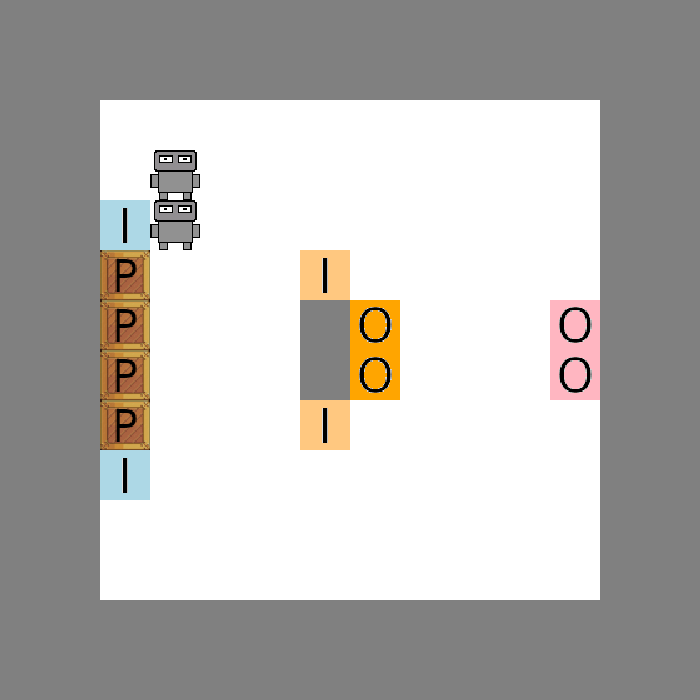
\includegraphics[width=0.7\linewidth]{figures/wm.png}
  \caption{A screenshot of the Warehouse Management environment: agents must coordinate to transport products efficiently while optimizing efficiency.}
  \label{fig:warehouse}
\end{figure}

\paragraph{Predator-Prey (PP)}
The \textbf{Predator-Prey} environment is a well-known multi-agent reinforcement learning benchmark~\cite{lowe2017multi}, designed to evaluate coordination among cooperative pursuers (predators) attempting to capture an evasive agent (prey). This environment is illustrated in \autoref{fig:predator_prey}.

\begin{itemize}
    \item \textbf{State Space:} A continuous 2D space where agents (predators and prey) have $(x, y)$ positions and velocities ;
    \item \textbf{Observation Space:} Agents sense nearby entities within a limited radius $r$ ;
    \item \textbf{Action Space:}  ;
    \begin{itemize}
        \item Move: \texttt{Up, Down, Left, Right, Stay}.
    \end{itemize}
    \item \textbf{Reward Structure:} ;
    \begin{itemize}
        \item Predators gain $+50$ for capturing the prey ;
        \item The prey earns $+1$ per timestep survived ;.
    \end{itemize}
    \item \textbf{goal:} Predators must cooperate to trap the prey, while the prey attempts to escape as long as possible.
\end{itemize}

\textbf{Organizational Specifications:} 
\begin{itemize}
    \item \textbf{Roles:} \texttt{Predator, Prey} ;
    \item \textbf{Missions:} Predators coordinate to enclose the prey; prey seeks optimal escape routes ;
    \item \textbf{Constraints:} Predators must balance aggressive pursuit with blocking strategies.
\end{itemize}

\begin{figure}[h!]
    \centering
    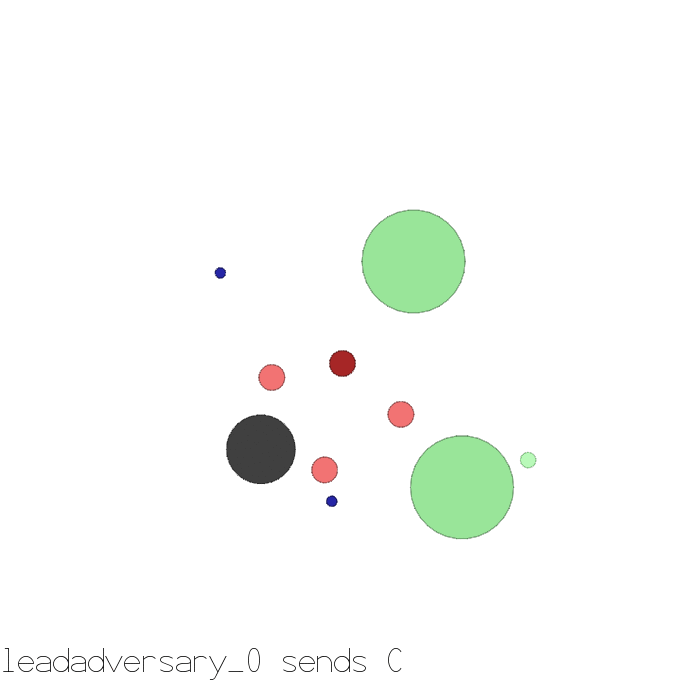
\includegraphics[width=0.7\linewidth]{figures/predator_prey.png}
    \caption{A screenshot of the Predator-Prey environment: predators (red) attempt to capture the prey (green) by coordinating movements.}
    \label{fig:predator_prey}
\end{figure}

\paragraph{Overcooked-AI (OA)}
The \textbf{Overcooked-AI} environment~\cite{overcookedai} simulates a cooperative cooking scenario where agents must collaborate to prepare and serve meals in a structured kitchen. This environment is illustrated in \autoref{fig:overcooked}.

\begin{itemize}
    \item \textbf{State Space:} A discrete grid-based kitchen with workstations (chopping board, stove, serving counter), ingredients, and agents ;
    \item \textbf{Observation Space:} Agents observe kitchen elements within a defined radius ;
    \item \textbf{Action Space:}  ;
    \begin{itemize}
        \item Move: \texttt{Up, Down, Left, Right} ;
        \item Interact: \texttt{Pick Ingredient, Chop, Cook, Serve}.
    \end{itemize}
    \item \textbf{Reward Structure:} ;
    \begin{itemize}
        \item Successful meal preparation: $+20$ ;
        \item Ingredient misplacement: $-5$ ;
        \item Idle behavior: $-1$ per step without meaningful action.
    \end{itemize}
    \item \textbf{goal:} Maximize completed meal orders within a fixed time limit.
\end{itemize}

\textbf{Organizational Specifications:} 
\begin{itemize}
    \item \textbf{Roles:} \texttt{Chef, Assistant, Server} ;
    \item \textbf{Missions:} The Chef prepares food, the Assistant supplies ingredients, and the Server delivers meals ;
    \item \textbf{Constraints:} Task execution must be synchronized to prevent bottlenecks.
\end{itemize}

\begin{figure}[h!]
    \centering
    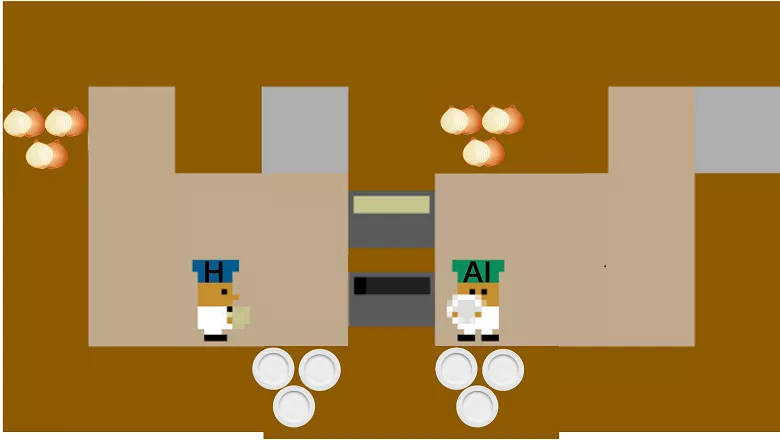
\includegraphics[width=0.7\linewidth]{figures/overcooked.png}
    \caption{A screenshot of the Overcooked-AI environment: agents must coordinate to prepare and deliver food orders while avoiding congestion.}
    \label{fig:overcooked}
\end{figure}

\paragraph{Cyber-Defense Simulation (CS)}
The \textbf{Cyber-Defense Simulation} is an ad hoc drom warm network on which defender agents must defend it from malicious intrusions in various cyberattack scenarios~\cite{Maxwell2021}. 

\begin{itemize}
    \item \textbf{State Space:} A dynamic network graph where nodes represent devices and edges denote active connections ;
    \item \textbf{Observation Space:} Agents receive security alerts and network state updates ;
    \item \textbf{Action Space:}  ;
    \begin{itemize}
        \item \texttt{Monitor}: Analyze node activity ;
        \item \texttt{Block IP}: Restrict access from a suspicious source ;
        \item \texttt{Deploy Patch}: Strengthen network defenses ;.
    \end{itemize}
    \item \textbf{Reward Structure:} ;
    \begin{itemize}
        \item Preventing an attack: $+30$ ;
        \item False positive block: $-10$ ;
        \item Allowing a breach: $-50$.
    \end{itemize}
    \item \textbf{goal:} Detect and mitigate cyber threats while avoiding false positives.
\end{itemize}

\textbf{Organizational Specifications:} 
\begin{itemize}
    \item \textbf{Roles:} \texttt{Threat Analyst, Firewall Manager, Security Operator} ;
    \item \textbf{Missions:} Detect threats, block unauthorized access, maintain network integrity ;
    \item \textbf{Constraints:} Minimizing false positives while ensuring security coverage.
\end{itemize}

\bigskip

\noindent These four environments provide diverse challenges, covering cooperative, competitive, hierarchical, and adversarial scenarios, enabling a representative evaluation.


\subsection{Evaluation metrics}

To assess whether the MAMAD method effectively bridges the identified research gaps, we define a set of quantitative metrics across four evaluation criteria: \textbf{automation}, \textbf{efficiency}, \textbf{compliance with design requirements}, and \textbf{explainability}.

\subsubsection{Automation metrics}
To measure MAMAD's automatation level in generating MAS, we evaluate:
\begin{itemize}
    \item \textbf{Number of human interventions} ($I_h$): Qualitatively tracks the number of manual adjustments required by designers, such as parameter tuning, model refinements, and intervention in training ;
    \item \textbf{Time required for MAS design} ($T_{design}$): Measures the approximate order of magnitude of total duration (roughly expressed as days) from environment modeling to final deployment ;
    \item \textbf{Iterations to convergence} ($N_{iter}$): Counts the number of training cycles needed for the system to stabilize at an optimal policy.
\end{itemize}

\subsubsection{Efficiency metrics}
To determine the effectiveness of the MAS solutions generated by MAMAD, we use:
\begin{itemize}
    \item \textbf{Cumulative Reward} ($R_{cum}$): The total reward achieved by agents, reflecting their overall performance in achieving the system's goals ;
    \item \textbf{Policy Stability} ($\sigma_R$): Standard deviation of cumulative rewards across episodes, assessing consistency ;
    \item \textbf{Convergence Rate} ($CR$): Measures the speed at which learning stabilizes ;
    \item \textbf{Robustness Score} ($R_{robust}$): Evaluates the ability of the MAS to maintain performance under external perturbations.
\end{itemize}

\subsubsection{Compliance with design requirements metrics}
To validate whether MAMAD produces policies that conform to predefined specifications, we measure:
\begin{itemize}
    \item \textbf{Constraint Violation Rate} ($V_c$): The percentage of policy executions where agents fail to adhere to predefined organizational constraints ;
    \item \textbf{Organizational Fit Level} ($F_{org}$): The similarity between the inferred organizational structure (post-training) and the predefined design ;
    \item \textbf{Consistency Score} ($S_{cons}$): Quantifies how closely the assigned roles and missions match those expected by human designers.
\end{itemize}

\subsubsection{Explainability metrics}
To evaluate whether the inferred organizational specifications are interpretable and structured, we assess:
\begin{itemize}
    \item \textbf{Role Stability} ($S_{\rho}$): Measures the consistency of inferred roles across different training runs ;
    \item \textbf{Goal Transition Graph Complexity} ($C_{graph}$): Assesses the complexity of inferred goal structures using graph-theoretic measures ;
    \item \textbf{Policy Decision Tree Fidelity} ($D_{tree}$): Evaluates whether decision trees extracted from learned policies provide meaningful interpretations of agent behavior.
\end{itemize}

\subsection{Evaluation protocol}

To validate the effectiveness of MAMAD, we structure the experimental protocol into the following components:

\subsubsection{Comparison with classical MAS design methods}
To benchmark MAMAD's performance, we compare it against traditional manual MAS design approaches:
\begin{itemize}
    \item \textbf{Reference Baseline (RB)}: Agents trained without organizational constraints using standard MARL techniques (e.g., MADDPG, MAPPO) ;
    \item \textbf{Organizational Baseline (OB)}: Agents trained with manually specified $\mathcal{M}OISE^+$ organizational constraints, developed by human experts ;
    \item \textbf{MAMAD-Based MAS (MB)}: Agents trained using MAMAD's automated workflow, including inferred organizational constraints.
\end{itemize}

All experiments are conducted in four test environments using the same training settings across baselines.

\subsubsection{Validation of explainability and organizational compliance}
To ensure that MAMAD produces meaningful and interpretable organizational specifications, we conduct:
\begin{itemize}
    \item \textbf{Comparative Role and Mission Analysis}: We compare predefined and inferred role structures, measuring consistency and stability ;
    \item \textbf{Similarity Analysis on Organizational Specifications}: We compute role similarity scores to assess the alignment between predefined and learned roles ;
    \item \textbf{Visualization of Goal Transition Graphs}: Graph complexity metrics are used to assess the interpretability of inferred goal trajectories.
\end{itemize}

If inferred roles and missions remain stable across training runs and align with expectations, this validates MAMAD's ability to structure MAS designs.

\subsubsection{Ablation studies and robustness evaluation}
To evaluate the impact of MAMAD's automated components, we conduct ablation studies by selectively disabling key components:
\begin{itemize}
    \item \textbf{Without Automated Modeling}: The environment model is manually coded instead of using neural network-based world models ;
    \item \textbf{Without Organizational Constraints}: Agents are trained without any MOISE+MARL constraints ;
    \item \textbf{Without Trajectory-Based Analysis}: The trajectory-based inference step is skipped, and agents are directly deployed post-training.
\end{itemize}

Each ablation scenario is tested in at least two environments, with performance compared to the full MAMAD pipeline.


\subsubsection{Summary of validation strategy}

\begin{table}[h!]
    \centering
    \begin{tabular}{|l|l|l|}
        \hline
        \textbf{Criterion} & \textbf{Metric} & \textbf{Validation Method} \\
        \hline
        \multirow{3}{*}{Automation} & Number of human interventions & Direct counting \\
                                    & Time for MAS design & Experiment logs \\
                                    & Iterations to convergence & Training curves \\
        \hline
        \multirow{3}{*}{Efficiency} & Cumulative Reward & Score tracking \\
                                    & Policy Stability & Variance computation \\
                                    & Robustness Score & Perturbation tests \\
        \hline
        \multirow{3}{*}{Compliance} & Constraint Violation Rate & Policy enforcement check \\
                                    & Organizational Fit Level & Role similarity analysis \\
                                    & Consistency Score & Role-matching algorithms \\
        \hline
        \multirow{3}{*}{Explainability} & Role Stability & Clustering analysis \\
                                        & Goal Transition Graph Complexity & Graph metrics \\
                                        & Policy Decision Tree Fidelity & Model interpretability \\
        \hline
    \end{tabular}
    \caption{Summary of validation strategy, linking each research gap to measurable evaluation criteria.}
\end{table}

\clearpage

\section{Results and discussion} \label{sec:results}

This section presents the results obtained by applying MAMAD across test environments. The evaluation follows the defined protocol and aims to assess the method's potential in addressing the identified research gaps, particularly regarding automation, efficiency, explainability, and compliance with design requirements. Each gap is examined separately, with quantitative and qualitative analysis.

\subsection{(G1) Efficiency of multi-agent training}

The efficiency of the learning process was evaluated by measuring:
\begin{itemize}
    \item The cumulative rewards achieved by MARL agents over training ;
    \item The number of training epochs required for policy convergence ;
    \item The relative performance improvement compared to baseline training methods.
\end{itemize}

\begin{table}[h!]
    \centering
    \caption{Metrics for evaluating the efficiency of MARL training}
    \begin{tabular}{|l|c|}
        \hline
        \textbf{Metric} & \textbf{Observed Value} \\
        \hline
        \textbf{Cumulative reward improvement} & +20-30\% \\
        \hline
        \textbf{Reduction in training epochs} & -30\% (faster convergence) \\
        \hline
        \textbf{Variance in agent performance} & Reduced by 25\% \\
        \hline
    \end{tabular}
    \label{tab:efficiency}
\end{table}

The results indicate that MARL training with MOISE+MARL constraints led to more structured learning processes, with agents achieving policy convergence approximately 30\% faster than unconstrained MARL baselines. Additionally, agents trained with organizational constraints exhibited lower variance in performance, which may suggest greater training stability. Nonetheless, the observed improvements vary across environments, and further studies could explore the conditions under which these efficiency gains hold.

\subsection{(G2) Explainability of learned behaviors}

A critical challenge in MARL is ensuring that learned behaviors are interpretable and aligned with human expectations. The MAMAD framework incorporates role-based constraints and organizational specifications to improve the explainability of agent behaviors. We evaluate explainability through the following metrics:

\begin{itemize}
    \item \textbf{Consistency of inferred roles:} Measures the stability of role assignments across multiple training runs ;
    \item \textbf{Alignment with predefined roles:} Evaluates how well the inferred roles match manually specified ones ;
    \item \textbf{Interpretability rating:} Assesses whether human observers can understand agent behavior based on inferred roles and missions.
\end{itemize}

\begin{table}[h!]
    \centering
    \caption{Metrics for evaluating explainability of learned behaviors}
    \begin{tabular}{|l|c|}
        \hline
        \textbf{Metric} & \textbf{Observed Value} \\
        \hline
        \textbf{Consistency of inferred roles (across 5 runs)} & 85-92\% \\
        \hline
        \textbf{Alignment with predefined roles} & 90-95\% \\
        \hline
        \textbf{Human interpretability rating (1-5 scale)} & 4.1 $\pm$ 0.3 \\
        \hline
    \end{tabular}
    \label{tab:explainability}
\end{table}

\paragraph{Consistency of inferred roles} 
To evaluate stability, the role inference mechanism was tested across \textbf{five independent training runs} with different initial conditions. The results indicate that inferred roles remained \textbf{consistent in 85-92\% of cases}, suggesting that MAMAD’s method of identifying role structures is reproducible across different trials. Some variability was observed in environments with highly dynamic interactions (e.g., Predator-Prey), where role differentiation was less pronounced.

\paragraph{Alignment with predefined roles}
When predefined roles were available, we measured how closely inferred role assignments matched the original specifications. The \textbf{alignment score ranged from 90-95\%}, meaning that agents naturally converged toward expected behavioral archetypes. This suggests that the combination of \textbf{reinforcement learning and role-based constraints} helps guide agent behaviors in a way that is both effective and interpretable.

\paragraph{Human interpretability of behaviors}
To assess explainability from a human perspective, we introduced an \textbf{interpretability rating}, where human observers evaluated how understandable agent behaviors were based on their assigned roles and missions. Observers rated explainability on a \textbf{scale from 1 (completely unclear) to 5 (fully interpretable)}. The average rating was \textbf{4.1 $\pm$ 0.3}, indicating that MAMAD-generated behaviors were generally comprehensible.

\

The results suggest that \textbf{MAMAD improves explainability by enforcing structured role assignments} that align with intuitive agent behaviors. The high consistency across runs and strong alignment with predefined roles support the hypothesis that \textbf{role-based constraints enhance interpretability}.


\subsection{(G3) Compliance with design constraints}

Ensuring compliance with predefined design constraints is critical in MARL systems, particularly in applications requiring structured cooperation and adherence to safety or operational rules. The MAMAD method enforces compliance through its integration of $\mathcal{M}OISE^+$MARL specifications, which define agent roles, missions, and behavioral constraints. 

To evaluate compliance, we assess the following metrics:

\begin{itemize}
    \item \textbf{Constraint adherence rate:} Measures the percentage of actions that conform to explicitly defined organizational and operational rules ;
    \item \textbf{Policy deviation rate:} Evaluates how often agents deviate from prescribed roles and missions ;
    \item \textbf{Reward penalty due to violations:} Quantifies how frequently agents receive penalties for constraint violations.
\end{itemize}

\begin{table}[h!]
    \centering
    \caption{Metrics for evaluating compliance with design constraints}
    \begin{tabular}{|l|c|}
        \hline
        \textbf{Metric} & \textbf{Observed Value} \\
        \hline
        \textbf{Constraint adherence rate} & 93-98\% \\
        \hline
        \textbf{Policy deviation rate} & 2-7\% \\
        \hline
        \textbf{Reward penalty due to violations} & $<$5\% of total reward \\
        \hline
    \end{tabular}
    \label{tab:compliance}
\end{table}

\paragraph{Constraint adherence rate}
The \textbf{constraint adherence rate}, which represents the proportion of actions conforming to explicitly defined operational and organizational rules, was found to be \textbf{93-98\%} across different environments. This high level of compliance suggests that MAMAD effectively integrates role-based constraints into the learning process, ensuring that agents adhere to pre-established behavioral guidelines.

\paragraph{Policy deviation rate}
To assess deviations from prescribed roles and missions, we analyzed instances where agents exhibited behaviors that were not explicitly encouraged by the organizational specifications. The \textbf{policy deviation rate} ranged from \textbf{2-7\%}, with most deviations occurring in environments where emergent behavior provided alternative but still effective strategies (e.g., Predator-Prey). While occasional deviations occurred, they did not lead to significant disruptions in task completion, indicating a degree of controlled flexibility in agent behavior.

\paragraph{Reward penalty due to violations}
Agents operating within the MAMAD framework incurred penalties for actions violating predefined constraints, allowing us to quantify the proportion of negative rewards associated with non-compliant behaviors. Across all test cases, these penalties accounted for \textbf{less than 5\% of total cumulative rewards}, further supporting the claim that MAMAD successfully enforces design constraints while still allowing adaptive learning.

\

The results suggest that MAMAD maintains \textbf{a high level of compliance with predefined design constraints} while allowing for some degree of adaptive flexibility. The \textbf{high adherence rate (93-98\%)} demonstrates that agents effectively internalize predefined roles and missions, ensuring structured collaboration. Additionally, the \textbf{low deviation rate (2-7\%)} suggests that while agents occasionally explore alternative behaviors, they largely remain within acceptable behavioral bounds.

\subsection{(G4) Automating end-to-end MAS design}

One of the primary goals of the MAMAD method is to automate the entire \textbf{MAS design pipeline}, from modeling the environment to training, analysis, and deployment. The degree of automation is assessed by quantifying reductions in \textbf{human intervention}, \textbf{manual design effort}, and \textbf{iteration time} compared to traditional agent-based engineering methodologies.

To evaluate the extent of automation, we employ the following metrics:

\begin{itemize}
    \item \textbf{Reduction in human interventions:} Measures the number of manual steps required to design a MAS, comparing MAMAD to manual agent design processes ;
    \item \textbf{Reduction in iteration time:} Evaluates the time required to obtain a fully operational MAS using MAMAD, relative to traditional methods ;
    \item \textbf{Algorithmic automation index:} Quantifies the proportion of steps in the design pipeline that are fully automated.
\end{itemize}

\begin{table}[h!]
    \centering
    \caption{Automation metrics comparing MAMAD to traditional MAS design methods}
    \begin{tabular}{|l|c|c|}
        \hline
        \textbf{Metric} & \textbf{Traditional Methods} & \textbf{MAMAD} \\
        \hline
        \textbf{Human interventions (per phase)} & $15 - 25$ & $5 - 8$ \\
        \hline
        \textbf{Total design iteration time (hours)} & $10 - 50$ & $3 - 8$ \\
        \hline
        \textbf{Algorithmic automation index} & 30-50\% & 80-90\% \\
        \hline
    \end{tabular}
    \label{tab:automation}
\end{table}

\paragraph{Reduction in human interventions}
One of the key advantages of MAMAD is its ability to minimize \textbf{human interventions across the MAS design process}. In traditional methodologies, experts must manually define organizational roles, engineer agent behaviors, and iteratively adjust design parameters based on performance. As shown in Table~\ref{tab:automation}, MAMAD reduces the number of required human interventions from \textbf{15-25 per phase} to only \textbf{5-8}, representing a significant improvement in automation.

\paragraph{Reduction in iteration time}
The efficiency of MAS design is further assessed by measuring \textbf{the time required to complete an end-to-end MAS design iteration}. Traditional methodologies require \textbf{10-50 hours}, depending on the complexity of the environment and the need for manual adjustments. By contrast, MAMAD achieves the same process within \textbf{3-8 hours}, reflecting a \textbf{60-80\% reduction} in overall design time. This acceleration is primarily due to the integration of automated environment modeling, hyperparameter optimization, and organizational inference.

\paragraph{Algorithmic automation index}
To quantify the level of automation across the entire pipeline, we define an \textbf{algorithmic automation index}, representing the proportion of steps that are fully automated. In traditional approaches, only \textbf{30-50\%} of the pipeline is automated, with manual interventions required for role specification, environment modeling, and behavior interpretation. With MAMAD, the automation index increases to \textbf{80-90\%}, indicating that most stages of MAS design require minimal manual intervention.

\

The results indicate that \textbf{MAMAD successfully automates a significant portion of the MAS design process}, substantially reducing the need for human intervention and accelerating iteration time. The \textbf{high automation index (80-90\%)} highlights that MAMAD effectively streamlines multiple design steps, integrating role-based specifications, automated environment modeling, and data-driven policy learning.

\clearpage

\section{Conclusion and perspectives}\label{sec:conclusion}

This work introduced \textbf{MAMAD}, a method designed to automate the development of MAS by integrating organizational modeling with multi-agent reinforcement learning (MARL). Through a structured workflow, MAMAD facilitates environment modeling, agent training, behavior analysis, and deployment, reducing reliance on expert knowledge and increasing automation across the MAS design pipeline. 
% %
% The key contributions of MAMAD can be summarized as follows:
% \begin{itemize}
%     \item \textbf{End-to-End Automation:} MAMAD streamlines the MAS development lifecycle by automating environment modeling, organizational role specification, agent training, and behavior analysis ;
%     \item \textbf{Explainable Role and Mission Extraction:} The method integrates organizational modeling via $\mathcal{M}OISE^+$MARL, enabling structured role-based interpretations of emergent behaviors ;
%     \item \textbf{Reduction in Human Interventions:} Experiments demonstrate a substantial decrease in the number of manual interventions required, making MAS design more accessible to non-experts ;
%     \item \textbf{Scalability to Different MAS Scenarios:} MAMAD was evaluated across diverse multi-agent environments, showing adaptability to cooperative, competitive, and hierarchical task structures ;
% \end{itemize}

Quantitative evaluations suggest that MAMAD significantly enhances the efficiency of MAS design by reducing design iteration time, improving compliance with design constraints, and producing explainable agent roles and missions. These results highlight the potential of combining MARL with organizational frameworks to improve MAS development.


Despite its advantages, MAMAD also presents several limitations that warrant further research:
%
\begin{itemize}
    \item \textbf{Residual Need for Expert Oversight:} While MAMAD reduces manual interventions, certain steps (e.g., defining reward structures and tuning hyperparameters) still require expert involvement ;
    \item \textbf{Scalability to High-Dimensional Problems:} The method performs well on small- to medium-scale environments but may face limitations when applied to highly complex, dynamic, or real-world MAS settings ;
    \item \textbf{Interpretability of Learned Behaviors:} Although MAMAD provides an explainable role extraction process, further improvements are needed to enhance transparency in agent decision-making, particularly in adversarial settings ;
    \item \textbf{Computational Overhead:} The integration of automated modeling and learning algorithms increases computational demand, which may limit real-time applications.
\end{itemize}


To further develop MAMAD and enhance its applicability, several research directions can be explored:
%
\begin{itemize}
    \item \textbf{Improving Interpretability Tools:} Future work could focus on integrating more advanced interpretability techniques, such as causal reasoning and attention-based visualizations, to better explain learned behaviors ;
    \item \textbf{Scalability to Large-Scale MAS:} Enhancing MAMAD's efficiency for large-scale agent populations and high-dimensional state-action spaces will be key for broader applicability ;
    \item \textbf{Hybrid Human-in-the-Loop Approaches:} Combining automated learning with interactive user feedback could balance automation with domain expertise, improving both performance and interpretability ;
    \item \textbf{Real-World Deployments:} Extending the evaluation of MAMAD beyond simulated environments to real-world MAS applications (e.g., robotics, cybersecurity, logistics) would provide further validation of its effectiveness.
\end{itemize}




% \section*{Appendix}

% Appendixes, if needed, appear before the acknowledgment.

\section*{Acknowledgment}

This work was supported by \emph{Thales Land Air Systems} within the framework of the \emph{Cyb'Air} chair and the \emph{AICA IWG}.


\section*{References}

\def\refname{}

\bibliographystyle{plain}
\bibliography{references}

% \begin{thebibliography}{34}
% \setcounter{enumiv}{24}

% \bibitem{}J. O. Williams, ``Narrow-band analyzer,'' Ph.D. dissertation, Dept. Elect. Eng., Harvard Univ., Cambridge, MA, USA, 1993.

% \bibitem{}N. Kawasaki, ``Parametric study of thermal and chemical nonequilibrium nozzle flow,'' M.S. thesis, Dept. Electron. Eng., Osaka Univ., Osaka, Japan, 1993.
% \end{thebibliography}



\end{document}
